\documentclass[1p]{elsarticle_modified}
%\bibliographystyle{elsarticle-num}

%\usepackage[colorlinks]{hyperref}
%\usepackage{abbrmath_seonhwa} %\Abb, \Ascr, \Acal ,\Abf, \Afrak
\usepackage{amsfonts}
\usepackage{amssymb}
\usepackage{amsmath}
\usepackage{amsthm}
\usepackage{scalefnt}
\usepackage{amsbsy}
\usepackage{kotex}
\usepackage{caption}
\usepackage{subfig}
\usepackage{color}
\usepackage{graphicx}
\usepackage{xcolor} %% white, black, red, green, blue, cyan, magenta, yellow
\usepackage{float}
\usepackage{setspace}
\usepackage{hyperref}

\usepackage{tikz}
\usetikzlibrary{arrows}

\usepackage{multirow}
\usepackage{array} % fixed length table
\usepackage{hhline}

%%%%%%%%%%%%%%%%%%%%%
\makeatletter
\renewcommand*\env@matrix[1][\arraystretch]{%
	\edef\arraystretch{#1}%
	\hskip -\arraycolsep
	\let\@ifnextchar\new@ifnextchar
	\array{*\c@MaxMatrixCols c}}
\makeatother %https://tex.stackexchange.com/questions/14071/how-can-i-increase-the-line-spacing-in-a-matrix
%%%%%%%%%%%%%%%

\usepackage[normalem]{ulem}

\newcommand{\msout}[1]{\ifmmode\text{\sout{\ensuremath{#1}}}\else\sout{#1}\fi}
%SOURCE: \msout is \stkout macro in https://tex.stackexchange.com/questions/20609/strikeout-in-math-mode

\newcommand{\cancel}[1]{
	\ifmmode
	{\color{red}\msout{#1}}
	\else
	{\color{red}\sout{#1}}
	\fi
}

\newcommand{\add}[1]{
	{\color{blue}\uwave{#1}}
}

\newcommand{\replace}[2]{
	\ifmmode
	{\color{red}\msout{#1}}{\color{blue}\uwave{#2}}
	\else
	{\color{red}\sout{#1}}{\color{blue}\uwave{#2}}
	\fi
}

\newcommand{\Sol}{\mathcal{S}} %segment
\newcommand{\D}{D} %diagram
\newcommand{\A}{\mathcal{A}} %arc


%%%%%%%%%%%%%%%%%%%%%%%%%%%%%5 test

\def\sl{\operatorname{\textup{SL}}(2,\Cbb)}
\def\psl{\operatorname{\textup{PSL}}(2,\Cbb)}
\def\quan{\mkern 1mu \triangleright \mkern 1mu}

\theoremstyle{definition}
\newtheorem{thm}{Theorem}[section]
\newtheorem{prop}[thm]{Proposition}
\newtheorem{lem}[thm]{Lemma}
\newtheorem{ques}[thm]{Question}
\newtheorem{cor}[thm]{Corollary}
\newtheorem{defn}[thm]{Definition}
\newtheorem{exam}[thm]{Example}
\newtheorem{rmk}[thm]{Remark}
\newtheorem{alg}[thm]{Algorithm}

\newcommand{\I}{\sqrt{-1}}
\begin{document}

%\begin{frontmatter}
%
%\title{Boundary parabolic representations of knots up to 8 crossings}
%
%%% Group authors per affiliation:
%\author{Yunhi Cho} 
%\address{Department of Mathematics, University of Seoul, Seoul, Korea}
%\ead{yhcho@uos.ac.kr}
%
%
%\author{Seonhwa Kim} %\fnref{s_kim}}
%\address{Center for Geometry and Physics, Institute for Basic Science, Pohang, 37673, Korea}
%\ead{ryeona17@ibs.re.kr}
%
%\author{Hyuk Kim}
%\address{Department of Mathematical Sciences, Seoul National University, Seoul 08826, Korea}
%\ead{hyukkim@snu.ac.kr}
%
%\author{Seokbeom Yoon}
%\address{Department of Mathematical Sciences, Seoul National University, Seoul, 08826,  Korea}
%\ead{sbyoon15@snu.ac.kr}
%
%\begin{abstract}
%We find all boundary parabolic representation of knots up to 8 crossings.
%
%\end{abstract}
%\begin{keyword}
%    \MSC[2010] 57M25 
%\end{keyword}
%
%\end{frontmatter}

%\linenumbers
%\tableofcontents
%
\newcommand\colored[1]{\textcolor{white}{\rule[-0.35ex]{0.8em}{1.4ex}}\kern-0.8em\color{red} #1}%
%\newcommand\colored[1]{\textcolor{white}{ #1}\kern-2.17ex	\textcolor{white}{ #1}\kern-1.81ex	\textcolor{white}{ #1}\kern-2.15ex\color{red}#1	}

{\Large $\underline{12a_{1250}~(K12a_{1250})}$}

\setlength{\tabcolsep}{10pt}
\renewcommand{\arraystretch}{1.6}
\vspace{1cm}\begin{tabular}{m{100pt}>{\centering\arraybackslash}m{274pt}}
\multirow{5}{120pt}{
	\centering
	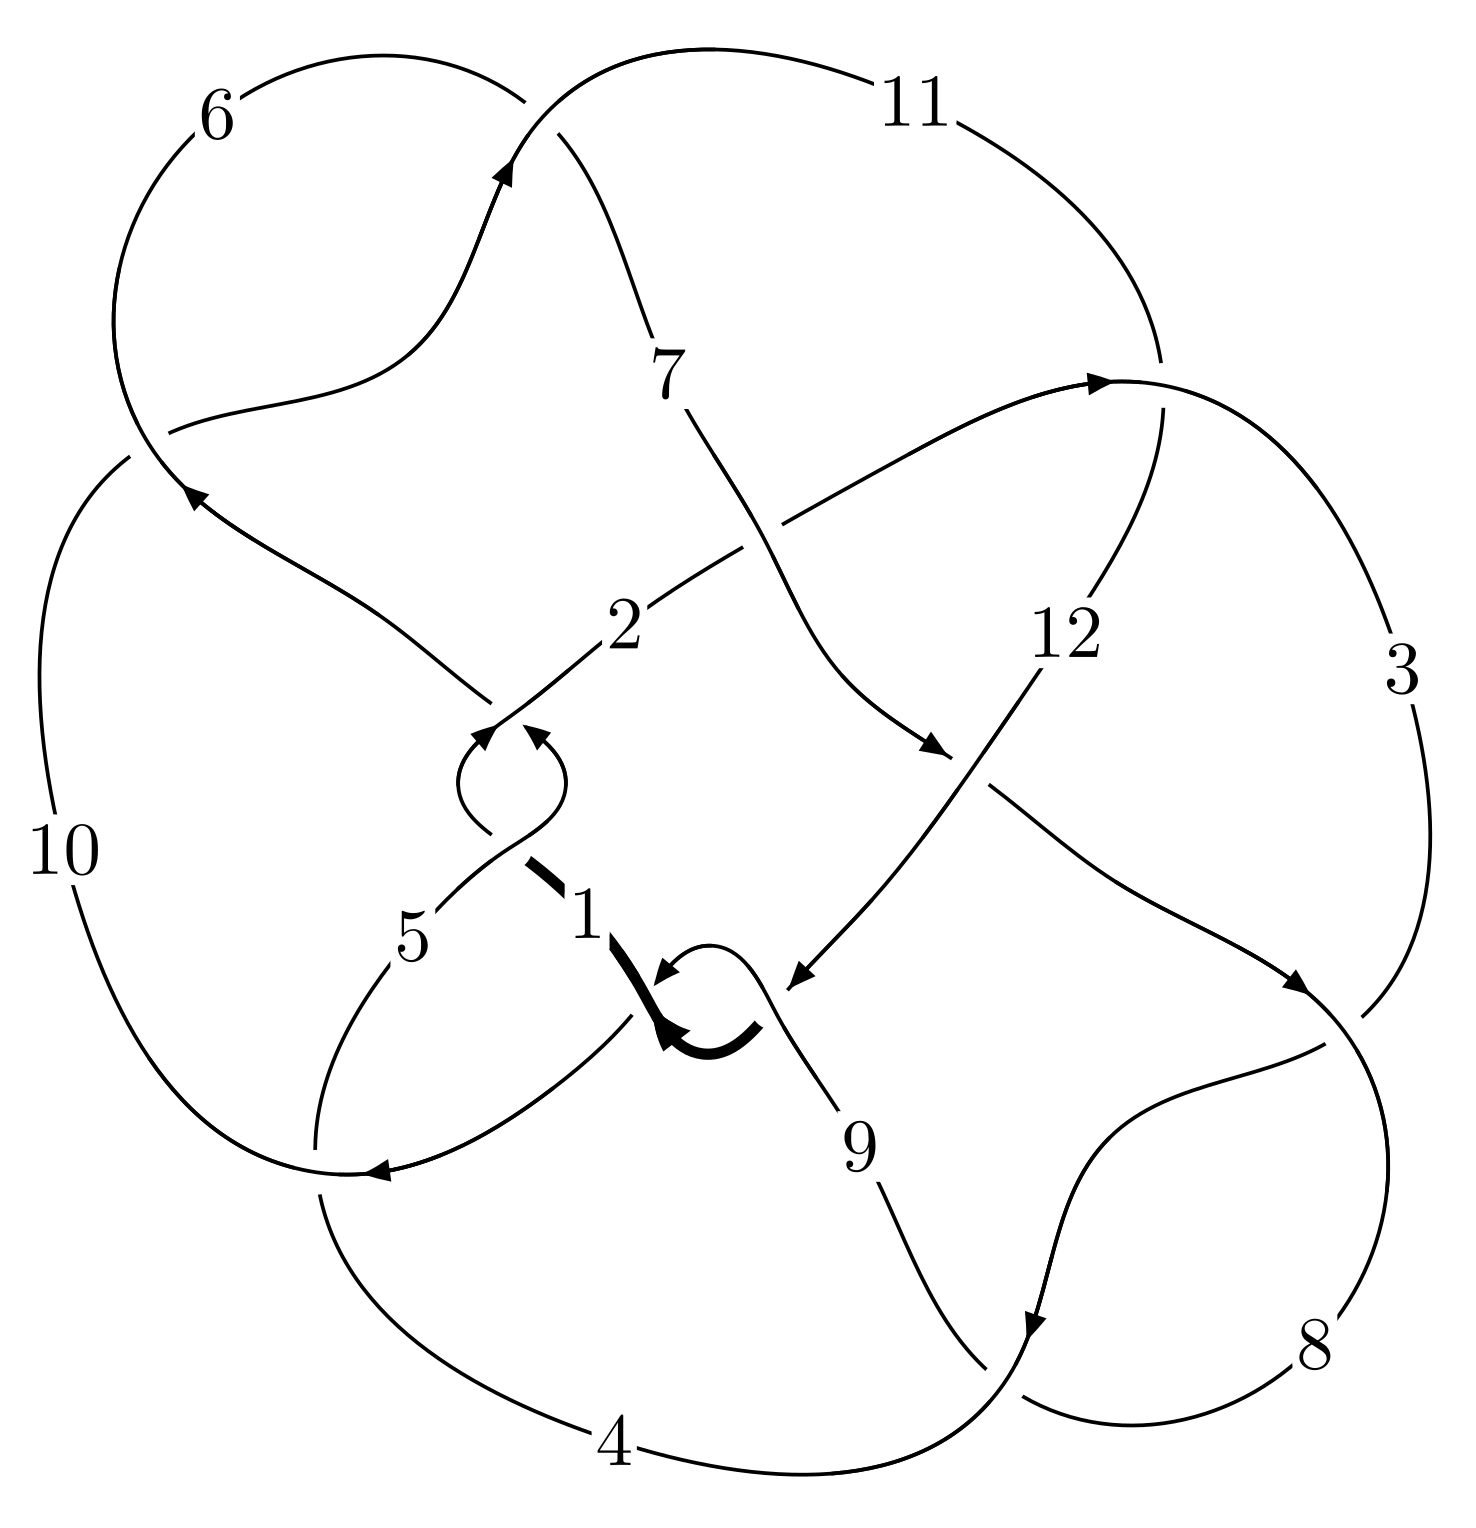
\includegraphics[width=112pt]{../../../GIT/diagram.site/Diagrams/png/2051_12a_1250.png}\\
\ \ \ A knot diagram\footnotemark}&
\allowdisplaybreaks
\textbf{Linearized knot diagam} \\
\cline{2-2}
 &
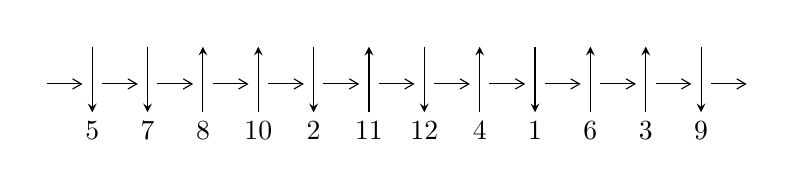
\begin{tikzpicture}[x=20pt, y=17pt]
	% nodes
	\node (C0) at (0, 0) {};
	\node (C1) at (1, 0) {};
	\node (C1U) at (1, +1) {};
	\node (C1D) at (1, -1) {5};

	\node (C2) at (2, 0) {};
	\node (C2U) at (2, +1) {};
	\node (C2D) at (2, -1) {7};

	\node (C3) at (3, 0) {};
	\node (C3U) at (3, +1) {};
	\node (C3D) at (3, -1) {8};

	\node (C4) at (4, 0) {};
	\node (C4U) at (4, +1) {};
	\node (C4D) at (4, -1) {10};

	\node (C5) at (5, 0) {};
	\node (C5U) at (5, +1) {};
	\node (C5D) at (5, -1) {2};

	\node (C6) at (6, 0) {};
	\node (C6U) at (6, +1) {};
	\node (C6D) at (6, -1) {11};

	\node (C7) at (7, 0) {};
	\node (C7U) at (7, +1) {};
	\node (C7D) at (7, -1) {12};

	\node (C8) at (8, 0) {};
	\node (C8U) at (8, +1) {};
	\node (C8D) at (8, -1) {4};

	\node (C9) at (9, 0) {};
	\node (C9U) at (9, +1) {};
	\node (C9D) at (9, -1) {1};

	\node (C10) at (10, 0) {};
	\node (C10U) at (10, +1) {};
	\node (C10D) at (10, -1) {6};

	\node (C11) at (11, 0) {};
	\node (C11U) at (11, +1) {};
	\node (C11D) at (11, -1) {3};

	\node (C12) at (12, 0) {};
	\node (C12U) at (12, +1) {};
	\node (C12D) at (12, -1) {9};
	\node (C13) at (13, 0) {};

	% arrows
	\draw[->,>={angle 60}]
	(C0) edge (C1) (C1) edge (C2) (C2) edge (C3) (C3) edge (C4) (C4) edge (C5) (C5) edge (C6) (C6) edge (C7) (C7) edge (C8) (C8) edge (C9) (C9) edge (C10) (C10) edge (C11) (C11) edge (C12) (C12) edge (C13) ;	\draw[->,>=stealth]
	(C1U) edge (C1D) (C2U) edge (C2D) (C3D) edge (C3U) (C4D) edge (C4U) (C5U) edge (C5D) (C6D) edge (C6U) (C7U) edge (C7D) (C8D) edge (C8U) (C9U) edge (C9D) (C10D) edge (C10U) (C11D) edge (C11U) (C12U) edge (C12D) ;
	\end{tikzpicture} \\
\hhline{~~} \\& 
\textbf{Solving Sequence} \\ \cline{2-2} 
 &
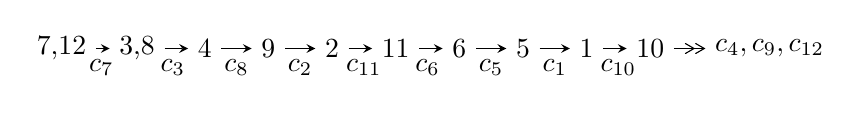
\begin{tikzpicture}[x=23pt, y=7pt]
	% node
	\node (A0) at (-1/8, 0) {7,12};
	\node (A1) at (17/16, 0) {3,8};
	\node (A2) at (17/8, 0) {4};
	\node (A3) at (25/8, 0) {9};
	\node (A4) at (33/8, 0) {2};
	\node (A5) at (41/8, 0) {11};
	\node (A6) at (49/8, 0) {6};
	\node (A7) at (57/8, 0) {5};
	\node (A8) at (65/8, 0) {1};
	\node (A9) at (73/8, 0) {10};
	\node (C1) at (1/2, -1) {$c_{7}$};
	\node (C2) at (13/8, -1) {$c_{3}$};
	\node (C3) at (21/8, -1) {$c_{8}$};
	\node (C4) at (29/8, -1) {$c_{2}$};
	\node (C5) at (37/8, -1) {$c_{11}$};
	\node (C6) at (45/8, -1) {$c_{6}$};
	\node (C7) at (53/8, -1) {$c_{5}$};
	\node (C8) at (61/8, -1) {$c_{1}$};
	\node (C9) at (69/8, -1) {$c_{10}$};
	\node (A10) at (11, 0) {$c_{4},c_{9},c_{12}$};

	% edge
	\draw[->,>=stealth]	
	(A0) edge (A1) (A1) edge (A2) (A2) edge (A3) (A3) edge (A4) (A4) edge (A5) (A5) edge (A6) (A6) edge (A7) (A7) edge (A8) (A8) edge (A9) ;
	\draw[->>,>={angle 60}]	
	(A9) edge (A10);
\end{tikzpicture} \\ 

\end{tabular} \\

\footnotetext{
The image of knot diagram is generated by the software ``\textbf{Draw programme}" developed by Andrew Bartholomew(\url{http://www.layer8.co.uk/maths/draw/index.htm\#Running-draw}), where we modified some parts for our purpose(\url{https://github.com/CATsTAILs/LinksPainter}).
}\phantom \\ \newline 
\centering \textbf{Ideals for irreducible components\footnotemark of $X_{\text{par}}$} 
 
\begin{align*}
I^u_{1}&=\langle 
b- u,\;7.70010\times10^{31} u^{26}-5.62456\times10^{31} u^{25}+\cdots+2.15871\times10^{31} a+1.22744\times10^{32},\;u^{27}- u^{26}+\cdots- u-1\rangle \\
I^u_{2}&=\langle 
4.84865\times10^{726} u^{109}-7.94449\times10^{726} u^{108}+\cdots+4.71721\times10^{727} b+2.09824\times10^{728},\\
\phantom{I^u_{2}}&\phantom{= \langle  }1.16970\times10^{728} u^{109}-2.33622\times10^{728} u^{108}+\cdots+4.71721\times10^{727} a-5.42261\times10^{729},\\
\phantom{I^u_{2}}&\phantom{= \langle  }u^{110}-2 u^{109}+\cdots-61 u+1\rangle \\
I^u_{3}&=\langle 
b+u,\;u^8+56 u^7-94 u^6+123 u^5+22 u^4-254 u^3+48 u^2+137 a+269 u-286,\\
\phantom{I^u_{3}}&\phantom{= \langle  }u^9- u^8+2 u^7+u^6-2 u^5- u^4+4 u^3- u^2- u-1\rangle \\
I^u_{4}&=\langle 
-1.58027\times10^{18} u^{19}-6.87073\times10^{17} u^{18}+\cdots+3.87707\times10^{18} b+3.02858\times10^{18},\\
\phantom{I^u_{4}}&\phantom{= \langle  }7.97216\times10^{18} u^{19}+6.43988\times10^{18} u^{18}+\cdots+3.87707\times10^{18} a-3.92152\times10^{19},\;u^{20}+u^{19}+\cdots-7 u-1\rangle \\
\\
\end{align*}
\raggedright * 4 irreducible components of $\dim_{\mathbb{C}}=0$, with total 166 representations.\\
\footnotetext{All coefficients of polynomials are rational numbers. But the coefficients are sometimes approximated in decimal forms when there is not enough margin.}
\newpage
\renewcommand{\arraystretch}{1}
\centering \section*{I. $I^u_{1}= \langle b- u,\;7.70\times10^{31} u^{26}-5.62\times10^{31} u^{25}+\cdots+2.16\times10^{31} a+1.23\times10^{32},\;u^{27}- u^{26}+\cdots- u-1 \rangle$}
\flushleft \textbf{(i) Arc colorings}\\
\begin{tabular}{m{7pt} m{180pt} m{7pt} m{180pt} }
\flushright $a_{7}=$&$\begin{pmatrix}1\\0\end{pmatrix}$ \\
\flushright $a_{12}=$&$\begin{pmatrix}0\\u\end{pmatrix}$ \\
\flushright $a_{3}=$&$\begin{pmatrix}-3.56698 u^{26}+2.60552 u^{25}+\cdots-4.88748 u-5.68596\\u\end{pmatrix}$ \\
\flushright $a_{8}=$&$\begin{pmatrix}1\\u^2\end{pmatrix}$ \\
\flushright $a_{4}=$&$\begin{pmatrix}-2.88044 u^{26}+2.25984 u^{25}+\cdots+0.640970 u-4.72449\\0.177619 u^{26}-0.100159 u^{25}+\cdots+2.02741 u+0.340863\end{pmatrix}$ \\
\flushright $a_{9}=$&$\begin{pmatrix}1.57118 u^{26}-0.212597 u^{25}+\cdots+20.1688 u+5.62807\\-0.688725 u^{26}+0.271933 u^{25}+\cdots-3.68073 u-1.38945\end{pmatrix}$ \\
\flushright $a_{2}=$&$\begin{pmatrix}-3.56698 u^{26}+2.60552 u^{25}+\cdots-3.88748 u-5.68596\\u\end{pmatrix}$ \\
\flushright $a_{11}=$&$\begin{pmatrix}-3.80911 u^{26}+1.86959 u^{25}+\cdots-11.4495 u-13.7172\\0.686544 u^{26}-0.345680 u^{25}+\cdots+5.52845 u+0.961469\end{pmatrix}$ \\
\flushright $a_{6}=$&$\begin{pmatrix}-4.77289 u^{26}+1.75400 u^{25}+\cdots-33.9661 u-4.39005\\1.32981 u^{26}-0.626906 u^{25}+\cdots+6.61049 u+2.74803\end{pmatrix}$ \\
\flushright $a_{5}=$&$\begin{pmatrix}-2.08988 u^{26}+1.15394 u^{25}+\cdots-6.43107 u-1.87197\\0.688725 u^{26}-0.271933 u^{25}+\cdots+3.68073 u+1.38945\end{pmatrix}$ \\
\flushright $a_{1}=$&$\begin{pmatrix}-3.89150 u^{26}+2.46159 u^{25}+\cdots-7.29656 u-6.52772\\1.20561 u^{26}-0.456383 u^{25}+\cdots+7.89661 u+2.30690\end{pmatrix}$ \\
\flushright $a_{10}=$&$\begin{pmatrix}1.36591 u^{26}-0.755536 u^{25}+\cdots+1.30324 u-3.58531\\-1.35273 u^{26}+0.596087 u^{25}+\cdots-6.04003 u-2.77861\end{pmatrix}$\\&\end{tabular}
\flushleft \textbf{(ii) Obstruction class $= -1$}\\~\\
\flushleft \textbf{(iii) Cusp Shapes $= 0.380648 u^{26}-0.165770 u^{25}+\cdots+7.21208 u-2.80163$}\\~\\
\newpage\renewcommand{\arraystretch}{1}
\flushleft \textbf{(iv) u-Polynomials at the component}\newline \\
\begin{tabular}{m{50pt}|m{274pt}}
Crossings & \hspace{64pt}u-Polynomials at each crossing \\
\hline $$\begin{aligned}c_{1},c_{5},c_{9}\\c_{12}\end{aligned}$$&$\begin{aligned}
&u^{27}+u^{26}+\cdots+7 u-1
\end{aligned}$\\
\hline $$\begin{aligned}c_{2},c_{7}\end{aligned}$$&$\begin{aligned}
&u^{27}- u^{26}+\cdots- u-1
\end{aligned}$\\
\hline $$\begin{aligned}c_{3},c_{6},c_{8}\\c_{10}\end{aligned}$$&$\begin{aligned}
&u^{27}- u^{26}+\cdots+2 u+1
\end{aligned}$\\
\hline $$\begin{aligned}c_{4}\end{aligned}$$&$\begin{aligned}
&u^{27}-21 u^{26}+\cdots-776 u+8
\end{aligned}$\\
\hline $$\begin{aligned}c_{11}\end{aligned}$$&$\begin{aligned}
&u^{27}-13 u^{26}+\cdots-444 u+72
\end{aligned}$\\
\hline
\end{tabular}\\~\\
\newpage\renewcommand{\arraystretch}{1}
\flushleft \textbf{(v) Riley Polynomials at the component}\newline \\
\begin{tabular}{m{50pt}|m{274pt}}
Crossings & \hspace{64pt}Riley Polynomials at each crossing \\
\hline $$\begin{aligned}c_{1},c_{5},c_{9}\\c_{12}\end{aligned}$$&$\begin{aligned}
&y^{27}-25 y^{26}+\cdots+45 y-1
\end{aligned}$\\
\hline $$\begin{aligned}c_{2},c_{7}\end{aligned}$$&$\begin{aligned}
&y^{27}-15 y^{26}+\cdots+5 y-1
\end{aligned}$\\
\hline $$\begin{aligned}c_{3},c_{6},c_{8}\\c_{10}\end{aligned}$$&$\begin{aligned}
&y^{27}-21 y^{26}+\cdots+6 y-1
\end{aligned}$\\
\hline $$\begin{aligned}c_{4}\end{aligned}$$&$\begin{aligned}
&y^{27}-7 y^{26}+\cdots+456672 y-64
\end{aligned}$\\
\hline $$\begin{aligned}c_{11}\end{aligned}$$&$\begin{aligned}
&y^{27}-7 y^{26}+\cdots+41040 y-5184
\end{aligned}$\\
\hline
\end{tabular}\\~\\
\newpage\flushleft \textbf{(vi) Complex Volumes and Cusp Shapes}
$$\begin{array}{c|c|c}  
\text{Solutions to }I^u_{1}& \I (\text{vol} + \sqrt{-1}CS) & \text{Cusp shape}\\
 \hline 
\begin{aligned}
u &= \phantom{-}0.781819 + 0.631176 I \\
a &= \phantom{-}0.929861 + 0.399699 I \\
b &= \phantom{-}0.781819 + 0.631176 I\end{aligned}
 & -3.28970 - 2.28835 I & -2.71013 + 3.35068 I \\ \hline\begin{aligned}
u &= \phantom{-}0.781819 - 0.631176 I \\
a &= \phantom{-}0.929861 - 0.399699 I \\
b &= \phantom{-}0.781819 - 0.631176 I\end{aligned}
 & -3.28970 + 2.28835 I & -2.71013 - 3.35068 I \\ \hline\begin{aligned}
u &= -0.892407\phantom{ +0.000000I} \\
a &= \phantom{-}0.974906\phantom{ +0.000000I} \\
b &= -0.892407\phantom{ +0.000000I}\end{aligned}
 & \phantom{-}10.2498\phantom{ +0.000000I} & \phantom{-}43.3390\phantom{ +0.000000I} \\ \hline\begin{aligned}
u &= \phantom{-}1.16370\phantom{ +0.000000I} \\
a &= -0.405849\phantom{ +0.000000I} \\
b &= \phantom{-}1.16370\phantom{ +0.000000I}\end{aligned}
 & -0.711699\phantom{ +0.000000I} & -7.17600\phantom{ +0.000000I} \\ \hline\begin{aligned}
u &= -1.149710 + 0.219773 I \\
a &= -0.803273 - 0.736758 I \\
b &= -1.149710 + 0.219773 I\end{aligned}
 & -8.27330 - 1.09335 I & -7.94541 - 0.68772 I \\ \hline\begin{aligned}
u &= -1.149710 - 0.219773 I \\
a &= -0.803273 + 0.736758 I \\
b &= -1.149710 - 0.219773 I\end{aligned}
 & -8.27330 + 1.09335 I & -7.94541 + 0.68772 I \\ \hline\begin{aligned}
u &= \phantom{-}1.091930 + 0.455489 I \\
a &= \phantom{-}0.278245 - 0.905101 I \\
b &= \phantom{-}1.091930 + 0.455489 I\end{aligned}
 & -9.40709 - 6.96260 I & -7.55252 + 5.81824 I \\ \hline\begin{aligned}
u &= \phantom{-}1.091930 - 0.455489 I \\
a &= \phantom{-}0.278245 + 0.905101 I \\
b &= \phantom{-}1.091930 - 0.455489 I\end{aligned}
 & -9.40709 + 6.96260 I & -7.55252 - 5.81824 I \\ \hline\begin{aligned}
u &= \phantom{-}0.710875 + 1.032870 I \\
a &= \phantom{-}0.012712 - 1.150810 I \\
b &= \phantom{-}0.710875 + 1.032870 I\end{aligned}
 & \phantom{-}3.58219 - 4.38995 I & \phantom{-}4.84018 + 4.14000 I \\ \hline\begin{aligned}
u &= \phantom{-}0.710875 - 1.032870 I \\
a &= \phantom{-}0.012712 + 1.150810 I \\
b &= \phantom{-}0.710875 - 1.032870 I\end{aligned}
 & \phantom{-}3.58219 + 4.38995 I & \phantom{-}4.84018 - 4.14000 I\\
 \hline 
 \end{array}$$\newpage$$\begin{array}{c|c|c}  
\text{Solutions to }I^u_{1}& \I (\text{vol} + \sqrt{-1}CS) & \text{Cusp shape}\\
 \hline 
\begin{aligned}
u &= -0.644156 + 0.368503 I \\
a &= -1.11178 + 1.61261 I \\
b &= -0.644156 + 0.368503 I\end{aligned}
 & -3.67889 + 11.52960 I & -3.14313 - 8.69788 I \\ \hline\begin{aligned}
u &= -0.644156 - 0.368503 I \\
a &= -1.11178 - 1.61261 I \\
b &= -0.644156 - 0.368503 I\end{aligned}
 & -3.67889 - 11.52960 I & -3.14313 + 8.69788 I \\ \hline\begin{aligned}
u &= \phantom{-}0.603990\phantom{ +0.000000I} \\
a &= -2.03134\phantom{ +0.000000I} \\
b &= \phantom{-}0.603990\phantom{ +0.000000I}\end{aligned}
 & \phantom{-}3.10146\phantom{ +0.000000I} & \phantom{-}2.60470\phantom{ +0.000000I} \\ \hline\begin{aligned}
u &= -0.285348 + 0.511101 I \\
a &= \phantom{-}0.308003 - 1.070990 I \\
b &= -0.285348 + 0.511101 I\end{aligned}
 & \phantom{-}0.056105 + 1.042570 I & \phantom{-}1.04906 - 6.21655 I \\ \hline\begin{aligned}
u &= -0.285348 - 0.511101 I \\
a &= \phantom{-}0.308003 + 1.070990 I \\
b &= -0.285348 - 0.511101 I\end{aligned}
 & \phantom{-}0.056105 - 1.042570 I & \phantom{-}1.04906 + 6.21655 I \\ \hline\begin{aligned}
u &= \phantom{-}0.515570 + 0.073824 I \\
a &= -1.12863 + 1.53832 I \\
b &= \phantom{-}0.515570 + 0.073824 I\end{aligned}
 & \phantom{-}2.12465 - 0.60492 I & \phantom{-}3.40248 - 0.28266 I \\ \hline\begin{aligned}
u &= \phantom{-}0.515570 - 0.073824 I \\
a &= -1.12863 - 1.53832 I \\
b &= \phantom{-}0.515570 - 0.073824 I\end{aligned}
 & \phantom{-}2.12465 + 0.60492 I & \phantom{-}3.40248 + 0.28266 I \\ \hline\begin{aligned}
u &= -1.13528 + 0.95643 I \\
a &= -0.461555 - 1.048120 I \\
b &= -1.13528 + 0.95643 I\end{aligned}
 & \phantom{-}8.36830 + 7.25793 I & \phantom{-}6.59980 - 4.89800 I \\ \hline\begin{aligned}
u &= -1.13528 - 0.95643 I \\
a &= -0.461555 + 1.048120 I \\
b &= -1.13528 - 0.95643 I\end{aligned}
 & \phantom{-}8.36830 - 7.25793 I & \phantom{-}6.59980 + 4.89800 I \\ \hline\begin{aligned}
u &= -0.167835 + 0.252267 I \\
a &= -2.61305 + 4.57834 I \\
b &= -0.167835 + 0.252267 I\end{aligned}
 & -0.84726 - 3.06637 I & -5.24785 - 2.81435 I\\
 \hline 
 \end{array}$$\newpage$$\begin{array}{c|c|c}  
\text{Solutions to }I^u_{1}& \I (\text{vol} + \sqrt{-1}CS) & \text{Cusp shape}\\
 \hline 
\begin{aligned}
u &= -0.167835 - 0.252267 I \\
a &= -2.61305 - 4.57834 I \\
b &= -0.167835 - 0.252267 I\end{aligned}
 & -0.84726 + 3.06637 I & -5.24785 + 2.81435 I \\ \hline\begin{aligned}
u &= \phantom{-}1.30742 + 1.18234 I \\
a &= \phantom{-}0.274985 - 0.859641 I \\
b &= \phantom{-}1.30742 + 1.18234 I\end{aligned}
 & -0.0304 - 19.1903 I & \phantom{-0.000000 -}0. + 9.60894 I \\ \hline\begin{aligned}
u &= \phantom{-}1.30742 - 1.18234 I \\
a &= \phantom{-}0.274985 + 0.859641 I \\
b &= \phantom{-}1.30742 - 1.18234 I\end{aligned}
 & -0.0304 + 19.1903 I & \phantom{-0.000000 } 0. - 9.60894 I \\ \hline\begin{aligned}
u &= -1.11928 + 1.55419 I \\
a &= -0.061254 - 0.676810 I \\
b &= -1.11928 + 1.55419 I\end{aligned}
 & -1.31722 + 8.02915 I & -2.07270 - 6.52162 I \\ \hline\begin{aligned}
u &= -1.11928 - 1.55419 I \\
a &= -0.061254 + 0.676810 I \\
b &= -1.11928 - 1.55419 I\end{aligned}
 & -1.31722 - 8.02915 I & -2.07270 + 6.52162 I \\ \hline\begin{aligned}
u &= -1.95578\phantom{ +0.000000I} \\
a &= -0.414695\phantom{ +0.000000I} \\
b &= -1.95578\phantom{ +0.000000I}\end{aligned}
 & -8.01906\phantom{ +0.000000I} & -12.6810\phantom{ +0.000000I} \\ \hline\begin{aligned}
u &= \phantom{-}2.26848\phantom{ +0.000000I} \\
a &= \phantom{-}0.628451\phantom{ +0.000000I} \\
b &= \phantom{-}2.26848\phantom{ +0.000000I}\end{aligned}
 & -5.51420\phantom{ +0.000000I} & \phantom{-0.000000 } 0\\
 \hline 
 \end{array}$$\newpage\newpage\renewcommand{\arraystretch}{1}
\centering \section*{II. $I^u_{2}= \langle 4.85\times10^{726} u^{109}-7.94\times10^{726} u^{108}+\cdots+4.72\times10^{727} b+2.10\times10^{728},\;1.17\times10^{728} u^{109}-2.34\times10^{728} u^{108}+\cdots+4.72\times10^{727} a-5.42\times10^{729},\;u^{110}-2 u^{109}+\cdots-61 u+1 \rangle$}
\flushleft \textbf{(i) Arc colorings}\\
\begin{tabular}{m{7pt} m{180pt} m{7pt} m{180pt} }
\flushright $a_{7}=$&$\begin{pmatrix}1\\0\end{pmatrix}$ \\
\flushright $a_{12}=$&$\begin{pmatrix}0\\u\end{pmatrix}$ \\
\flushright $a_{3}=$&$\begin{pmatrix}-2.47964 u^{109}+4.95256 u^{108}+\cdots-3207.39 u+114.954\\-0.102786 u^{109}+0.168415 u^{108}+\cdots+104.323 u-4.44806\end{pmatrix}$ \\
\flushright $a_{8}=$&$\begin{pmatrix}1\\u^2\end{pmatrix}$ \\
\flushright $a_{4}=$&$\begin{pmatrix}-2.57837 u^{109}+5.11495 u^{108}+\cdots-3105.13 u+110.499\\-0.109476 u^{109}+0.179933 u^{108}+\cdots+102.283 u-4.41300\end{pmatrix}$ \\
\flushright $a_{9}=$&$\begin{pmatrix}-9.61748 u^{109}+18.8705 u^{108}+\cdots-8470.02 u+238.697\\1.30572 u^{109}-2.51884 u^{108}+\cdots+785.576 u-17.1918\end{pmatrix}$ \\
\flushright $a_{2}=$&$\begin{pmatrix}-2.58243 u^{109}+5.12097 u^{108}+\cdots-3103.06 u+110.506\\-0.102786 u^{109}+0.168415 u^{108}+\cdots+104.323 u-4.44806\end{pmatrix}$ \\
\flushright $a_{11}=$&$\begin{pmatrix}6.11025 u^{109}-12.0451 u^{108}+\cdots+6254.55 u-195.782\\-0.430403 u^{109}+0.856393 u^{108}+\cdots-406.059 u+10.7574\end{pmatrix}$ \\
\flushright $a_{6}=$&$\begin{pmatrix}13.7340 u^{109}-26.8864 u^{108}+\cdots+12163.2 u-371.524\\-0.153525 u^{109}+0.289259 u^{108}+\cdots-155.930 u+7.46005\end{pmatrix}$ \\
\flushright $a_{5}=$&$\begin{pmatrix}21.7236 u^{109}-42.5002 u^{108}+\cdots+18797.6 u-552.054\\-1.19225 u^{109}+2.28448 u^{108}+\cdots-714.350 u+19.3249\end{pmatrix}$ \\
\flushright $a_{1}=$&$\begin{pmatrix}10.1698 u^{109}-19.9510 u^{108}+\cdots+9792.89 u-324.122\\0.780072 u^{109}-1.47552 u^{108}+\cdots+241.270 u+0.659459\end{pmatrix}$ \\
\flushright $a_{10}=$&$\begin{pmatrix}-18.6242 u^{109}+36.7385 u^{108}+\cdots-17618.2 u+537.624\\1.04694 u^{109}-2.02223 u^{108}+\cdots+826.486 u-22.9158\end{pmatrix}$\\&\end{tabular}
\flushleft \textbf{(ii) Obstruction class $= -1$}\\~\\
\flushleft \textbf{(iii) Cusp Shapes $= -1.39827 u^{109}+2.80537 u^{108}+\cdots-1473.20 u+34.2235$}\\~\\
\newpage\renewcommand{\arraystretch}{1}
\flushleft \textbf{(iv) u-Polynomials at the component}\newline \\
\begin{tabular}{m{50pt}|m{274pt}}
Crossings & \hspace{64pt}u-Polynomials at each crossing \\
\hline $$\begin{aligned}c_{1},c_{5},c_{9}\\c_{12}\end{aligned}$$&$\begin{aligned}
&u^{110}-37 u^{108}+\cdots-596 u+229
\end{aligned}$\\
\hline $$\begin{aligned}c_{2},c_{7}\end{aligned}$$&$\begin{aligned}
&u^{110}-2 u^{109}+\cdots-61 u+1
\end{aligned}$\\
\hline $$\begin{aligned}c_{3},c_{6},c_{8}\\c_{10}\end{aligned}$$&$\begin{aligned}
&u^{110}+u^{109}+\cdots+2947 u+199
\end{aligned}$\\
\hline $$\begin{aligned}c_{4}\end{aligned}$$&$\begin{aligned}
&(u^{55}+10 u^{54}+\cdots+8 u-1)^{2}
\end{aligned}$\\
\hline $$\begin{aligned}c_{11}\end{aligned}$$&$\begin{aligned}
&(u^{55}+6 u^{54}+\cdots+262 u+67)^{2}
\end{aligned}$\\
\hline
\end{tabular}\\~\\
\newpage\renewcommand{\arraystretch}{1}
\flushleft \textbf{(v) Riley Polynomials at the component}\newline \\
\begin{tabular}{m{50pt}|m{274pt}}
Crossings & \hspace{64pt}Riley Polynomials at each crossing \\
\hline $$\begin{aligned}c_{1},c_{5},c_{9}\\c_{12}\end{aligned}$$&$\begin{aligned}
&y^{110}-74 y^{109}+\cdots-2941542 y+52441
\end{aligned}$\\
\hline $$\begin{aligned}c_{2},c_{7}\end{aligned}$$&$\begin{aligned}
&y^{110}+8 y^{109}+\cdots-995 y+1
\end{aligned}$\\
\hline $$\begin{aligned}c_{3},c_{6},c_{8}\\c_{10}\end{aligned}$$&$\begin{aligned}
&y^{110}-71 y^{109}+\cdots-1508869 y+39601
\end{aligned}$\\
\hline $$\begin{aligned}c_{4}\end{aligned}$$&$\begin{aligned}
&(y^{55}+12 y^{54}+\cdots+236 y-1)^{2}
\end{aligned}$\\
\hline $$\begin{aligned}c_{11}\end{aligned}$$&$\begin{aligned}
&(y^{55}-20 y^{54}+\cdots+72932 y-4489)^{2}
\end{aligned}$\\
\hline
\end{tabular}\\~\\
\newpage\flushleft \textbf{(vi) Complex Volumes and Cusp Shapes}
$$\begin{array}{c|c|c}  
\text{Solutions to }I^u_{2}& \I (\text{vol} + \sqrt{-1}CS) & \text{Cusp shape}\\
 \hline 
\begin{aligned}
u &= -0.998893\phantom{ +0.000000I} \\
a &= -0.886698\phantom{ +0.000000I} \\
b &= -1.97821\phantom{ +0.000000I}\end{aligned}
 & -5.09057\phantom{ +0.000000I} & \phantom{-0.000000 } 0 \\ \hline\begin{aligned}
u &= -0.612762 + 0.750100 I \\
a &= \phantom{-}0.116640 - 1.014820 I \\
b &= \phantom{-}0.310391 + 0.813099 I\end{aligned}
 & \phantom{-}0.43264 + 4.10654 I & \phantom{-0.000000 } 0 \\ \hline\begin{aligned}
u &= -0.612762 - 0.750100 I \\
a &= \phantom{-}0.116640 + 1.014820 I \\
b &= \phantom{-}0.310391 - 0.813099 I\end{aligned}
 & \phantom{-}0.43264 - 4.10654 I & \phantom{-0.000000 } 0 \\ \hline\begin{aligned}
u &= -0.919737 + 0.556530 I \\
a &= -0.418031 - 1.172860 I \\
b &= -1.31673 + 1.11908 I\end{aligned}
 & -4.79048 + 12.57190 I & \phantom{-0.000000 } 0 \\ \hline\begin{aligned}
u &= -0.919737 - 0.556530 I \\
a &= -0.418031 + 1.172860 I \\
b &= -1.31673 - 1.11908 I\end{aligned}
 & -4.79048 - 12.57190 I & \phantom{-0.000000 } 0 \\ \hline\begin{aligned}
u &= \phantom{-}0.750183 + 0.770595 I \\
a &= -0.312632 + 0.823794 I \\
b &= -1.28027 - 1.36796 I\end{aligned}
 & -2.93335 - 2.67192 I & \phantom{-0.000000 } 0 \\ \hline\begin{aligned}
u &= \phantom{-}0.750183 - 0.770595 I \\
a &= -0.312632 - 0.823794 I \\
b &= -1.28027 + 1.36796 I\end{aligned}
 & -2.93335 + 2.67192 I & \phantom{-0.000000 } 0 \\ \hline\begin{aligned}
u &= \phantom{-}0.865133 + 0.669573 I \\
a &= \phantom{-}0.33802 - 1.57490 I \\
b &= \phantom{-}0.659251 + 0.966888 I\end{aligned}
 & \phantom{-}2.74486 - 4.81034 I & \phantom{-0.000000 } 0 \\ \hline\begin{aligned}
u &= \phantom{-}0.865133 - 0.669573 I \\
a &= \phantom{-}0.33802 + 1.57490 I \\
b &= \phantom{-}0.659251 - 0.966888 I\end{aligned}
 & \phantom{-}2.74486 + 4.81034 I & \phantom{-0.000000 } 0 \\ \hline\begin{aligned}
u &= \phantom{-}1.095580 + 0.042016 I \\
a &= \phantom{-}0.726760 + 1.014680 I \\
b &= \phantom{-}0.299331 + 0.204670 I\end{aligned}
 & -5.73179 - 5.61364 I & \phantom{-0.000000 } 0\\
 \hline 
 \end{array}$$\newpage$$\begin{array}{c|c|c}  
\text{Solutions to }I^u_{2}& \I (\text{vol} + \sqrt{-1}CS) & \text{Cusp shape}\\
 \hline 
\begin{aligned}
u &= \phantom{-}1.095580 - 0.042016 I \\
a &= \phantom{-}0.726760 - 1.014680 I \\
b &= \phantom{-}0.299331 - 0.204670 I\end{aligned}
 & -5.73179 + 5.61364 I & \phantom{-0.000000 } 0 \\ \hline\begin{aligned}
u &= \phantom{-}0.403309 + 0.807250 I \\
a &= -0.18776 - 1.50293 I \\
b &= \phantom{-}0.768789 + 0.929711 I\end{aligned}
 & \phantom{-}3.55445 - 4.03607 I & \phantom{-0.000000 } 0 \\ \hline\begin{aligned}
u &= \phantom{-}0.403309 - 0.807250 I \\
a &= -0.18776 + 1.50293 I \\
b &= \phantom{-}0.768789 - 0.929711 I\end{aligned}
 & \phantom{-}3.55445 + 4.03607 I & \phantom{-0.000000 } 0 \\ \hline\begin{aligned}
u &= \phantom{-}0.800426 + 0.358042 I \\
a &= -0.778741 + 1.108750 I \\
b &= \phantom{-}0.116547 - 0.222950 I\end{aligned}
 & \phantom{-}2.22016 - 0.68767 I & \phantom{-0.000000 } 0 \\ \hline\begin{aligned}
u &= \phantom{-}0.800426 - 0.358042 I \\
a &= -0.778741 - 1.108750 I \\
b &= \phantom{-}0.116547 + 0.222950 I\end{aligned}
 & \phantom{-}2.22016 + 0.68767 I & \phantom{-0.000000 } 0 \\ \hline\begin{aligned}
u &= \phantom{-}0.310391 + 0.813099 I \\
a &= \phantom{-}1.044060 - 0.449729 I \\
b &= -0.612762 + 0.750100 I\end{aligned}
 & \phantom{-}0.43264 + 4.10654 I & \phantom{-0.000000 } 0 \\ \hline\begin{aligned}
u &= \phantom{-}0.310391 - 0.813099 I \\
a &= \phantom{-}1.044060 + 0.449729 I \\
b &= -0.612762 - 0.750100 I\end{aligned}
 & \phantom{-}0.43264 - 4.10654 I & \phantom{-0.000000 } 0 \\ \hline\begin{aligned}
u &= \phantom{-}0.778176 + 0.373657 I \\
a &= -0.222898 + 0.908749 I \\
b &= -0.734460 - 0.894698 I\end{aligned}
 & -3.57918 - 3.06316 I & \phantom{-0.000000 } 0 \\ \hline\begin{aligned}
u &= \phantom{-}0.778176 - 0.373657 I \\
a &= -0.222898 - 0.908749 I \\
b &= -0.734460 + 0.894698 I\end{aligned}
 & -3.57918 + 3.06316 I & \phantom{-0.000000 } 0 \\ \hline\begin{aligned}
u &= \phantom{-}0.476407 + 1.045930 I \\
a &= \phantom{-}0.272044 - 0.568787 I \\
b &= -1.14858 + 1.39599 I\end{aligned}
 & \phantom{-}5.29292 - 4.11535 I & \phantom{-0.000000 } 0\\
 \hline 
 \end{array}$$\newpage$$\begin{array}{c|c|c}  
\text{Solutions to }I^u_{2}& \I (\text{vol} + \sqrt{-1}CS) & \text{Cusp shape}\\
 \hline 
\begin{aligned}
u &= \phantom{-}0.476407 - 1.045930 I \\
a &= \phantom{-}0.272044 + 0.568787 I \\
b &= -1.14858 - 1.39599 I\end{aligned}
 & \phantom{-}5.29292 + 4.11535 I & \phantom{-0.000000 } 0 \\ \hline\begin{aligned}
u &= \phantom{-}0.685571 + 0.923676 I \\
a &= -0.012161 + 1.122410 I \\
b &= -1.09417 - 1.14531 I\end{aligned}
 & \phantom{-}0.28959 - 9.04527 I & \phantom{-0.000000 } 0 \\ \hline\begin{aligned}
u &= \phantom{-}0.685571 - 0.923676 I \\
a &= -0.012161 - 1.122410 I \\
b &= -1.09417 + 1.14531 I\end{aligned}
 & \phantom{-}0.28959 + 9.04527 I & \phantom{-0.000000 } 0 \\ \hline\begin{aligned}
u &= -1.128550 + 0.253990 I \\
a &= \phantom{-}0.425568 + 0.390150 I \\
b &= \phantom{-}0.720258 - 0.243099 I\end{aligned}
 & -2.84990 + 0.29345 I & \phantom{-0.000000 } 0 \\ \hline\begin{aligned}
u &= -1.128550 - 0.253990 I \\
a &= \phantom{-}0.425568 - 0.390150 I \\
b &= \phantom{-}0.720258 + 0.243099 I\end{aligned}
 & -2.84990 - 0.29345 I & \phantom{-0.000000 } 0 \\ \hline\begin{aligned}
u &= -0.734460 + 0.894698 I \\
a &= -0.135378 + 0.684525 I \\
b &= \phantom{-}0.778176 - 0.373657 I\end{aligned}
 & -3.57918 + 3.06316 I & \phantom{-0.000000 } 0 \\ \hline\begin{aligned}
u &= -0.734460 - 0.894698 I \\
a &= -0.135378 - 0.684525 I \\
b &= \phantom{-}0.778176 + 0.373657 I\end{aligned}
 & -3.57918 - 3.06316 I & \phantom{-0.000000 } 0 \\ \hline\begin{aligned}
u &= \phantom{-}0.659251 + 0.966888 I \\
a &= -0.15376 - 1.49791 I \\
b &= \phantom{-}0.865133 + 0.669573 I\end{aligned}
 & \phantom{-}2.74486 - 4.81034 I & \phantom{-0.000000 } 0 \\ \hline\begin{aligned}
u &= \phantom{-}0.659251 - 0.966888 I \\
a &= -0.15376 + 1.49791 I \\
b &= \phantom{-}0.865133 - 0.669573 I\end{aligned}
 & \phantom{-}2.74486 + 4.81034 I & \phantom{-0.000000 } 0 \\ \hline\begin{aligned}
u &= -0.736806 + 0.367349 I \\
a &= \phantom{-}0.35529 + 1.54642 I \\
b &= \phantom{-}0.88136 - 1.24598 I\end{aligned}
 & \phantom{-}0.51004 + 5.45734 I & \phantom{-0.000000 } 0\\
 \hline 
 \end{array}$$\newpage$$\begin{array}{c|c|c}  
\text{Solutions to }I^u_{2}& \I (\text{vol} + \sqrt{-1}CS) & \text{Cusp shape}\\
 \hline 
\begin{aligned}
u &= -0.736806 - 0.367349 I \\
a &= \phantom{-}0.35529 - 1.54642 I \\
b &= \phantom{-}0.88136 + 1.24598 I\end{aligned}
 & \phantom{-}0.51004 - 5.45734 I & \phantom{-0.000000 } 0 \\ \hline\begin{aligned}
u &= -1.19982\phantom{ +0.000000I} \\
a &= \phantom{-}0.983271\phantom{ +0.000000I} \\
b &= \phantom{-}0.755437\phantom{ +0.000000I}\end{aligned}
 & -2.52587\phantom{ +0.000000I} & \phantom{-0.000000 } 0 \\ \hline\begin{aligned}
u &= \phantom{-}1.031690 + 0.617279 I \\
a &= -1.00449 + 1.18519 I \\
b &= -1.185780 - 0.516929 I\end{aligned}
 & \phantom{-}2.64974 - 1.27843 I & \phantom{-0.000000 } 0 \\ \hline\begin{aligned}
u &= \phantom{-}1.031690 - 0.617279 I \\
a &= -1.00449 - 1.18519 I \\
b &= -1.185780 + 0.516929 I\end{aligned}
 & \phantom{-}2.64974 + 1.27843 I & \phantom{-0.000000 } 0 \\ \hline\begin{aligned}
u &= \phantom{-}0.768789 + 0.929711 I \\
a &= \phantom{-}0.116846 - 1.126900 I \\
b &= \phantom{-}0.403309 + 0.807250 I\end{aligned}
 & \phantom{-}3.55445 - 4.03607 I & \phantom{-0.000000 } 0 \\ \hline\begin{aligned}
u &= \phantom{-}0.768789 - 0.929711 I \\
a &= \phantom{-}0.116846 + 1.126900 I \\
b &= \phantom{-}0.403309 - 0.807250 I\end{aligned}
 & \phantom{-}3.55445 + 4.03607 I & \phantom{-0.000000 } 0 \\ \hline\begin{aligned}
u &= -0.235929 + 0.757530 I \\
a &= \phantom{-}0.242037 - 1.144280 I \\
b &= -0.71885 + 1.37533 I\end{aligned}
 & \phantom{-}1.135820 - 0.205465 I & \phantom{-0.000000 } 0 \\ \hline\begin{aligned}
u &= -0.235929 - 0.757530 I \\
a &= \phantom{-}0.242037 + 1.144280 I \\
b &= -0.71885 - 1.37533 I\end{aligned}
 & \phantom{-}1.135820 + 0.205465 I & \phantom{-0.000000 } 0 \\ \hline\begin{aligned}
u &= -0.399940 + 1.157640 I \\
a &= -0.189094 - 0.717679 I \\
b &= \phantom{-}0.91748 + 1.35195 I\end{aligned}
 & \phantom{-}6.13336 + 4.50289 I & \phantom{-0.000000 } 0 \\ \hline\begin{aligned}
u &= -0.399940 - 1.157640 I \\
a &= -0.189094 + 0.717679 I \\
b &= \phantom{-}0.91748 - 1.35195 I\end{aligned}
 & \phantom{-}6.13336 - 4.50289 I & \phantom{-0.000000 } 0\\
 \hline 
 \end{array}$$\newpage$$\begin{array}{c|c|c}  
\text{Solutions to }I^u_{2}& \I (\text{vol} + \sqrt{-1}CS) & \text{Cusp shape}\\
 \hline 
\begin{aligned}
u &= \phantom{-}0.598936 + 0.485246 I \\
a &= -1.10106 + 0.89206 I \\
b &= \phantom{-}0.598936 - 0.485246 I\end{aligned}
 & \phantom{-}3.02407\phantom{ +0.000000I} & \phantom{-0.000000 } 0 \\ \hline\begin{aligned}
u &= \phantom{-}0.598936 - 0.485246 I \\
a &= -1.10106 - 0.89206 I \\
b &= \phantom{-}0.598936 + 0.485246 I\end{aligned}
 & \phantom{-}3.02407\phantom{ +0.000000I} & \phantom{-0.000000 } 0 \\ \hline\begin{aligned}
u &= \phantom{-}0.720258 + 0.243099 I \\
a &= -0.582371 + 0.657801 I \\
b &= -1.128550 - 0.253990 I\end{aligned}
 & -2.84990 - 0.29345 I & \phantom{-0.000000 } 0 \\ \hline\begin{aligned}
u &= \phantom{-}0.720258 - 0.243099 I \\
a &= -0.582371 - 0.657801 I \\
b &= -1.128550 + 0.253990 I\end{aligned}
 & -2.84990 + 0.29345 I & \phantom{-0.000000 } 0 \\ \hline\begin{aligned}
u &= \phantom{-}0.755437\phantom{ +0.000000I} \\
a &= -1.56167\phantom{ +0.000000I} \\
b &= -1.19982\phantom{ +0.000000I}\end{aligned}
 & -2.52587\phantom{ +0.000000I} & -18.3860\phantom{ +0.000000I} \\ \hline\begin{aligned}
u &= \phantom{-}0.958529 + 0.798223 I \\
a &= \phantom{-}0.367727 - 0.784409 I \\
b &= \phantom{-}1.72624 + 1.25070 I\end{aligned}
 & -3.70148 - 2.64555 I & \phantom{-0.000000 } 0 \\ \hline\begin{aligned}
u &= \phantom{-}0.958529 - 0.798223 I \\
a &= \phantom{-}0.367727 + 0.784409 I \\
b &= \phantom{-}1.72624 - 1.25070 I\end{aligned}
 & -3.70148 + 2.64555 I & \phantom{-0.000000 } 0 \\ \hline\begin{aligned}
u &= -0.777794 + 1.015010 I \\
a &= \phantom{-}0.395951 + 0.516708 I \\
b &= -0.777794 - 1.015010 I\end{aligned}
 & \phantom{-}9.31937\phantom{ +0.000000I} & \phantom{-0.000000 } 0 \\ \hline\begin{aligned}
u &= -0.777794 - 1.015010 I \\
a &= \phantom{-}0.395951 - 0.516708 I \\
b &= -0.777794 + 1.015010 I\end{aligned}
 & \phantom{-}9.31937\phantom{ +0.000000I} & \phantom{-0.000000 } 0 \\ \hline\begin{aligned}
u &= -0.651259 + 0.284105 I \\
a &= \phantom{-}0.56779 - 2.19424 I \\
b &= \phantom{-}0.311295 - 0.145457 I\end{aligned}
 & \phantom{-}0.80420 + 4.80655 I & \phantom{-0.000000 } 0. - 9.09767 I\\
 \hline 
 \end{array}$$\newpage$$\begin{array}{c|c|c}  
\text{Solutions to }I^u_{2}& \I (\text{vol} + \sqrt{-1}CS) & \text{Cusp shape}\\
 \hline 
\begin{aligned}
u &= -0.651259 - 0.284105 I \\
a &= \phantom{-}0.56779 + 2.19424 I \\
b &= \phantom{-}0.311295 + 0.145457 I\end{aligned}
 & \phantom{-}0.80420 - 4.80655 I & \phantom{-0.000000 -}0. + 9.09767 I \\ \hline\begin{aligned}
u &= -1.185780 + 0.516929 I \\
a &= \phantom{-}1.06665 + 0.97326 I \\
b &= \phantom{-}1.031690 - 0.617279 I\end{aligned}
 & \phantom{-}2.64974 + 1.27843 I & \phantom{-0.000000 } 0 \\ \hline\begin{aligned}
u &= -1.185780 - 0.516929 I \\
a &= \phantom{-}1.06665 - 0.97326 I \\
b &= \phantom{-}1.031690 + 0.617279 I\end{aligned}
 & \phantom{-}2.64974 - 1.27843 I & \phantom{-0.000000 } 0 \\ \hline\begin{aligned}
u &= -0.186211 + 0.650498 I \\
a &= \phantom{-}1.139500 + 0.549929 I \\
b &= \phantom{-}0.050931 - 1.383410 I\end{aligned}
 & -1.67519 + 3.37319 I & \phantom{-0.000000 } 0. - 1.85055 I \\ \hline\begin{aligned}
u &= -0.186211 - 0.650498 I \\
a &= \phantom{-}1.139500 - 0.549929 I \\
b &= \phantom{-}0.050931 + 1.383410 I\end{aligned}
 & -1.67519 - 3.37319 I & \phantom{-0.000000 -}0. + 1.85055 I \\ \hline\begin{aligned}
u &= -0.334305 + 0.582293 I \\
a &= -0.068999 + 1.362830 I \\
b &= \phantom{-}1.34936 - 1.20783 I\end{aligned}
 & \phantom{-}1.22183 + 3.59271 I & \phantom{-}4.52275 - 8.70901 I \\ \hline\begin{aligned}
u &= -0.334305 - 0.582293 I \\
a &= -0.068999 - 1.362830 I \\
b &= \phantom{-}1.34936 + 1.20783 I\end{aligned}
 & \phantom{-}1.22183 - 3.59271 I & \phantom{-}4.52275 + 8.70901 I \\ \hline\begin{aligned}
u &= -1.35619\phantom{ +0.000000I} \\
a &= -1.03010\phantom{ +0.000000I} \\
b &= \phantom{-}0.0351718\phantom{ +0.000000I}\end{aligned}
 & \phantom{-}3.28865\phantom{ +0.000000I} & \phantom{-0.000000 } 0 \\ \hline\begin{aligned}
u &= -0.621797 + 0.148820 I \\
a &= \phantom{-}1.26656 - 1.44413 I \\
b &= \phantom{-}0.233671 - 0.407335 I\end{aligned}
 & -1.08485 + 2.66555 I & -6.08010 - 4.56372 I \\ \hline\begin{aligned}
u &= -0.621797 - 0.148820 I \\
a &= \phantom{-}1.26656 + 1.44413 I \\
b &= \phantom{-}0.233671 + 0.407335 I\end{aligned}
 & -1.08485 - 2.66555 I & -6.08010 + 4.56372 I\\
 \hline 
 \end{array}$$\newpage$$\begin{array}{c|c|c}  
\text{Solutions to }I^u_{2}& \I (\text{vol} + \sqrt{-1}CS) & \text{Cusp shape}\\
 \hline 
\begin{aligned}
u &= \phantom{-}0.050931 + 1.383410 I \\
a &= -0.476306 + 0.394428 I \\
b &= -0.186211 - 0.650498 I\end{aligned}
 & -1.67519 - 3.37319 I & \phantom{-0.000000 } 0 \\ \hline\begin{aligned}
u &= \phantom{-}0.050931 - 1.383410 I \\
a &= -0.476306 - 0.394428 I \\
b &= -0.186211 + 0.650498 I\end{aligned}
 & -1.67519 + 3.37319 I & \phantom{-0.000000 } 0 \\ \hline\begin{aligned}
u &= -1.369060 + 0.309100 I \\
a &= -0.079909 - 0.455040 I \\
b &= -0.457160 - 0.144522 I\end{aligned}
 & -5.63317 + 1.03399 I & \phantom{-0.000000 } 0 \\ \hline\begin{aligned}
u &= -1.369060 - 0.309100 I \\
a &= -0.079909 + 0.455040 I \\
b &= -0.457160 + 0.144522 I\end{aligned}
 & -5.63317 - 1.03399 I & \phantom{-0.000000 } 0 \\ \hline\begin{aligned}
u &= -0.457160 + 0.144522 I \\
a &= -0.873399 + 1.032580 I \\
b &= -1.369060 - 0.309100 I\end{aligned}
 & -5.63317 - 1.03399 I & -11.65387 + 4.39006 I \\ \hline\begin{aligned}
u &= -0.457160 - 0.144522 I \\
a &= -0.873399 - 1.032580 I \\
b &= -1.369060 + 0.309100 I\end{aligned}
 & -5.63317 + 1.03399 I & -11.65387 - 4.39006 I \\ \hline\begin{aligned}
u &= \phantom{-}0.88136 + 1.24598 I \\
a &= \phantom{-}0.225679 + 0.825663 I \\
b &= -0.736806 - 0.367349 I\end{aligned}
 & \phantom{-}0.51004 - 5.45734 I & \phantom{-0.000000 } 0 \\ \hline\begin{aligned}
u &= \phantom{-}0.88136 - 1.24598 I \\
a &= \phantom{-}0.225679 - 0.825663 I \\
b &= -0.736806 + 0.367349 I\end{aligned}
 & \phantom{-}0.51004 + 5.45734 I & \phantom{-0.000000 } 0 \\ \hline\begin{aligned}
u &= \phantom{-}0.233671 + 0.407335 I \\
a &= -2.61356 - 0.09350 I \\
b &= -0.621797 - 0.148820 I\end{aligned}
 & -1.08485 - 2.66555 I & -6.08010 + 4.56372 I \\ \hline\begin{aligned}
u &= \phantom{-}0.233671 - 0.407335 I \\
a &= -2.61356 + 0.09350 I \\
b &= -0.621797 + 0.148820 I\end{aligned}
 & -1.08485 + 2.66555 I & -6.08010 - 4.56372 I\\
 \hline 
 \end{array}$$\newpage$$\begin{array}{c|c|c}  
\text{Solutions to }I^u_{2}& \I (\text{vol} + \sqrt{-1}CS) & \text{Cusp shape}\\
 \hline 
\begin{aligned}
u &= -0.71885 + 1.37533 I \\
a &= \phantom{-}0.017188 - 0.597731 I \\
b &= -0.235929 + 0.757530 I\end{aligned}
 & \phantom{-}1.135820 - 0.205465 I & \phantom{-0.000000 } 0 \\ \hline\begin{aligned}
u &= -0.71885 - 1.37533 I \\
a &= \phantom{-}0.017188 + 0.597731 I \\
b &= -0.235929 - 0.757530 I\end{aligned}
 & \phantom{-}1.135820 + 0.205465 I & \phantom{-0.000000 } 0 \\ \hline\begin{aligned}
u &= \phantom{-}0.40372 + 1.51303 I \\
a &= -0.118661 + 0.535099 I \\
b &= \phantom{-}0.89017 - 1.87925 I\end{aligned}
 & \phantom{-}1.42772 - 9.18102 I & \phantom{-0.000000 } 0 \\ \hline\begin{aligned}
u &= \phantom{-}0.40372 - 1.51303 I \\
a &= -0.118661 - 0.535099 I \\
b &= \phantom{-}0.89017 + 1.87925 I\end{aligned}
 & \phantom{-}1.42772 + 9.18102 I & \phantom{-0.000000 } 0 \\ \hline\begin{aligned}
u &= \phantom{-}1.19083 + 1.04289 I \\
a &= -0.325712 + 0.983158 I \\
b &= -1.11259 - 1.13543 I\end{aligned}
 & \phantom{-}5.13513 - 12.91180 I & \phantom{-0.000000 } 0 \\ \hline\begin{aligned}
u &= \phantom{-}1.19083 - 1.04289 I \\
a &= -0.325712 - 0.983158 I \\
b &= -1.11259 + 1.13543 I\end{aligned}
 & \phantom{-}5.13513 + 12.91180 I & \phantom{-0.000000 } 0 \\ \hline\begin{aligned}
u &= -1.09417 + 1.14531 I \\
a &= \phantom{-}0.109630 + 0.807747 I \\
b &= \phantom{-}0.685571 - 0.923676 I\end{aligned}
 & \phantom{-}0.28959 + 9.04527 I & \phantom{-0.000000 } 0 \\ \hline\begin{aligned}
u &= -1.09417 - 1.14531 I \\
a &= \phantom{-}0.109630 - 0.807747 I \\
b &= \phantom{-}0.685571 + 0.923676 I\end{aligned}
 & \phantom{-}0.28959 - 9.04527 I & \phantom{-0.000000 } 0 \\ \hline\begin{aligned}
u &= -1.11259 + 1.13543 I \\
a &= \phantom{-}0.248773 + 1.000870 I \\
b &= \phantom{-}1.19083 - 1.04289 I\end{aligned}
 & \phantom{-}5.13513 + 12.91180 I & \phantom{-0.000000 } 0 \\ \hline\begin{aligned}
u &= -1.11259 - 1.13543 I \\
a &= \phantom{-}0.248773 - 1.000870 I \\
b &= \phantom{-}1.19083 + 1.04289 I\end{aligned}
 & \phantom{-}5.13513 - 12.91180 I & \phantom{-0.000000 } 0\\
 \hline 
 \end{array}$$\newpage$$\begin{array}{c|c|c}  
\text{Solutions to }I^u_{2}& \I (\text{vol} + \sqrt{-1}CS) & \text{Cusp shape}\\
 \hline 
\begin{aligned}
u &= \phantom{-}0.91748 + 1.35195 I \\
a &= \phantom{-}0.346032 - 0.435642 I \\
b &= -0.399940 + 1.157640 I\end{aligned}
 & \phantom{-}6.13336 + 4.50289 I & \phantom{-0.000000 } 0 \\ \hline\begin{aligned}
u &= \phantom{-}0.91748 - 1.35195 I \\
a &= \phantom{-}0.346032 + 0.435642 I \\
b &= -0.399940 - 1.157640 I\end{aligned}
 & \phantom{-}6.13336 - 4.50289 I & \phantom{-0.000000 } 0 \\ \hline\begin{aligned}
u &= \phantom{-}0.299331 + 0.204670 I \\
a &= \phantom{-}3.49343 + 1.42719 I \\
b &= \phantom{-}1.095580 + 0.042016 I\end{aligned}
 & -5.73179 - 5.61364 I & -4.53556 + 5.12202 I \\ \hline\begin{aligned}
u &= \phantom{-}0.299331 - 0.204670 I \\
a &= \phantom{-}3.49343 - 1.42719 I \\
b &= \phantom{-}1.095580 - 0.042016 I\end{aligned}
 & -5.73179 + 5.61364 I & -4.53556 - 5.12202 I \\ \hline\begin{aligned}
u &= -0.85657 + 1.41626 I \\
a &= \phantom{-}0.013688 + 0.755530 I \\
b &= \phantom{-}0.57663 - 1.59776 I\end{aligned}
 & -0.05548 + 8.46629 I & \phantom{-0.000000 } 0 \\ \hline\begin{aligned}
u &= -0.85657 - 1.41626 I \\
a &= \phantom{-}0.013688 - 0.755530 I \\
b &= \phantom{-}0.57663 + 1.59776 I\end{aligned}
 & -0.05548 - 8.46629 I & \phantom{-0.000000 } 0 \\ \hline\begin{aligned}
u &= \phantom{-}0.311295 + 0.145457 I \\
a &= -1.29063 - 4.50569 I \\
b &= -0.651259 - 0.284105 I\end{aligned}
 & \phantom{-}0.80420 - 4.80655 I & -1.31755 + 9.09767 I \\ \hline\begin{aligned}
u &= \phantom{-}0.311295 - 0.145457 I \\
a &= -1.29063 + 4.50569 I \\
b &= -0.651259 + 0.284105 I\end{aligned}
 & \phantom{-}0.80420 + 4.80655 I & -1.31755 - 9.09767 I \\ \hline\begin{aligned}
u &= \phantom{-}0.57663 + 1.59776 I \\
a &= \phantom{-}0.131446 + 0.724481 I \\
b &= -0.85657 - 1.41626 I\end{aligned}
 & -0.05548 - 8.46629 I & \phantom{-0.000000 } 0 \\ \hline\begin{aligned}
u &= \phantom{-}0.57663 - 1.59776 I \\
a &= \phantom{-}0.131446 - 0.724481 I \\
b &= -0.85657 + 1.41626 I\end{aligned}
 & -0.05548 + 8.46629 I & \phantom{-0.000000 } 0\\
 \hline 
 \end{array}$$\newpage$$\begin{array}{c|c|c}  
\text{Solutions to }I^u_{2}& \I (\text{vol} + \sqrt{-1}CS) & \text{Cusp shape}\\
 \hline 
\begin{aligned}
u &= -1.31673 + 1.11908 I \\
a &= -0.140282 - 0.761785 I \\
b &= -0.919737 + 0.556530 I\end{aligned}
 & -4.79048 + 12.57190 I & \phantom{-0.000000 } 0 \\ \hline\begin{aligned}
u &= -1.31673 - 1.11908 I \\
a &= -0.140282 + 0.761785 I \\
b &= -0.919737 - 0.556530 I\end{aligned}
 & -4.79048 - 12.57190 I & \phantom{-0.000000 } 0 \\ \hline\begin{aligned}
u &= \phantom{-}0.116547 + 0.222950 I \\
a &= -4.02294 + 2.47338 I \\
b &= \phantom{-}0.800426 - 0.358042 I\end{aligned}
 & \phantom{-}2.22016 + 0.68767 I & \phantom{-}3.24172 + 1.08060 I \\ \hline\begin{aligned}
u &= \phantom{-}0.116547 - 0.222950 I \\
a &= -4.02294 - 2.47338 I \\
b &= \phantom{-}0.800426 + 0.358042 I\end{aligned}
 & \phantom{-}2.22016 - 0.68767 I & \phantom{-}3.24172 - 1.08060 I \\ \hline\begin{aligned}
u &= -1.14858 + 1.39599 I \\
a &= -0.248844 - 0.314256 I \\
b &= \phantom{-}0.476407 + 1.045930 I\end{aligned}
 & \phantom{-}5.29292 - 4.11535 I & \phantom{-0.000000 } 0 \\ \hline\begin{aligned}
u &= -1.14858 - 1.39599 I \\
a &= -0.248844 + 0.314256 I \\
b &= \phantom{-}0.476407 - 1.045930 I\end{aligned}
 & \phantom{-}5.29292 + 4.11535 I & \phantom{-0.000000 } 0 \\ \hline\begin{aligned}
u &= \phantom{-}1.34936 + 1.20783 I \\
a &= -0.134425 + 0.487742 I \\
b &= -0.334305 - 0.582293 I\end{aligned}
 & \phantom{-}1.22183 - 3.59271 I & \phantom{-0.000000 } 0 \\ \hline\begin{aligned}
u &= \phantom{-}1.34936 - 1.20783 I \\
a &= -0.134425 - 0.487742 I \\
b &= -0.334305 + 0.582293 I\end{aligned}
 & \phantom{-}1.22183 + 3.59271 I & \phantom{-0.000000 } 0 \\ \hline\begin{aligned}
u &= -1.28027 + 1.36796 I \\
a &= \phantom{-}0.170112 + 0.476297 I \\
b &= \phantom{-}0.750183 - 0.770595 I\end{aligned}
 & -2.93335 + 2.67192 I & \phantom{-0.000000 } 0 \\ \hline\begin{aligned}
u &= -1.28027 - 1.36796 I \\
a &= \phantom{-}0.170112 - 0.476297 I \\
b &= \phantom{-}0.750183 + 0.770595 I\end{aligned}
 & -2.93335 - 2.67192 I & \phantom{-0.000000 } 0\\
 \hline 
 \end{array}$$\newpage$$\begin{array}{c|c|c}  
\text{Solutions to }I^u_{2}& \I (\text{vol} + \sqrt{-1}CS) & \text{Cusp shape}\\
 \hline 
\begin{aligned}
u &= \phantom{-}0.0767307 + 0.0358246 I \\
a &= \phantom{-}1.43169 - 8.47092 I \\
b &= \phantom{-}1.32363 + 1.40196 I\end{aligned}
 & -1.41309 - 4.17051 I & -10.11255 + 0.98560 I \\ \hline\begin{aligned}
u &= \phantom{-}0.0767307 - 0.0358246 I \\
a &= \phantom{-}1.43169 + 8.47092 I \\
b &= \phantom{-}1.32363 - 1.40196 I\end{aligned}
 & -1.41309 + 4.17051 I & -10.11255 - 0.98560 I \\ \hline\begin{aligned}
u &= \phantom{-}1.32363 + 1.40196 I \\
a &= -0.078616 - 0.369041 I \\
b &= \phantom{-}0.0767307 + 0.0358246 I\end{aligned}
 & -1.41309 - 4.17051 I & \phantom{-0.000000 } 0 \\ \hline\begin{aligned}
u &= \phantom{-}1.32363 - 1.40196 I \\
a &= -0.078616 + 0.369041 I \\
b &= \phantom{-}0.0767307 - 0.0358246 I\end{aligned}
 & -1.41309 + 4.17051 I & \phantom{-0.000000 } 0 \\ \hline\begin{aligned}
u &= \phantom{-}0.0351718\phantom{ +0.000000I} \\
a &= \phantom{-}39.7196\phantom{ +0.000000I} \\
b &= -1.35619\phantom{ +0.000000I}\end{aligned}
 & \phantom{-}3.28865\phantom{ +0.000000I} & \phantom{-}1.98690\phantom{ +0.000000I} \\ \hline\begin{aligned}
u &= -1.97821\phantom{ +0.000000I} \\
a &= -0.447737\phantom{ +0.000000I} \\
b &= -0.998893\phantom{ +0.000000I}\end{aligned}
 & -5.09057\phantom{ +0.000000I} & \phantom{-0.000000 } 0 \\ \hline\begin{aligned}
u &= \phantom{-}0.89017 + 1.87925 I \\
a &= -0.192398 + 0.365177 I \\
b &= \phantom{-}0.40372 - 1.51303 I\end{aligned}
 & \phantom{-}1.42772 + 9.18102 I & \phantom{-0.000000 } 0 \\ \hline\begin{aligned}
u &= \phantom{-}0.89017 - 1.87925 I \\
a &= -0.192398 - 0.365177 I \\
b &= \phantom{-}0.40372 + 1.51303 I\end{aligned}
 & \phantom{-}1.42772 - 9.18102 I & \phantom{-0.000000 } 0 \\ \hline\begin{aligned}
u &= \phantom{-}1.72624 + 1.25070 I \\
a &= \phantom{-}0.245604 - 0.443464 I \\
b &= \phantom{-}0.958529 + 0.798223 I\end{aligned}
 & -3.70148 - 2.64555 I & \phantom{-0.000000 } 0 \\ \hline\begin{aligned}
u &= \phantom{-}1.72624 - 1.25070 I \\
a &= \phantom{-}0.245604 + 0.443464 I \\
b &= \phantom{-}0.958529 - 0.798223 I\end{aligned}
 & -3.70148 + 2.64555 I & \phantom{-0.000000 } 0\\
 \hline 
 \end{array}$$\newpage\newpage\renewcommand{\arraystretch}{1}
\centering \section*{III. $I^u_{3}= \langle b+u,\;u^8+56 u^7+\cdots+137 a-286,\;u^9- u^8+\cdots- u-1 \rangle$}
\flushleft \textbf{(i) Arc colorings}\\
\begin{tabular}{m{7pt} m{180pt} m{7pt} m{180pt} }
\flushright $a_{7}=$&$\begin{pmatrix}1\\0\end{pmatrix}$ \\
\flushright $a_{12}=$&$\begin{pmatrix}0\\u\end{pmatrix}$ \\
\flushright $a_{3}=$&$\begin{pmatrix}-0.00729927 u^{8}-0.408759 u^{7}+\cdots-1.96350 u+2.08759\\- u\end{pmatrix}$ \\
\flushright $a_{8}=$&$\begin{pmatrix}1\\u^2\end{pmatrix}$ \\
\flushright $a_{4}=$&$\begin{pmatrix}-0.291971 u^{8}-0.350365 u^{7}+\cdots-2.54015 u+2.50365\\0.102190 u^{8}-0.277372 u^{7}+\cdots-1.51095 u-0.226277\end{pmatrix}$ \\
\flushright $a_{9}=$&$\begin{pmatrix}0.547445 u^{8}-0.343066 u^{7}+\cdots+0.262774 u-1.56934\\-0.372263 u^{8}+0.153285 u^{7}+\cdots-0.138686 u-0.532847\end{pmatrix}$ \\
\flushright $a_{2}=$&$\begin{pmatrix}-0.00729927 u^{8}-0.408759 u^{7}+\cdots-2.96350 u+2.08759\\- u\end{pmatrix}$ \\
\flushright $a_{11}=$&$\begin{pmatrix}1.82482 u^{8}-2.81022 u^{7}+\cdots-6.12409 u-0.897810\\0.284672 u^{8}-0.0583942 u^{7}+\cdots+0.576642 u-0.416058\end{pmatrix}$ \\
\flushright $a_{6}=$&$\begin{pmatrix}-1.09489 u^{8}+1.68613 u^{7}+\cdots+4.47445 u+0.138686\\0.0218978 u^{8}+0.226277 u^{7}+\cdots+0.890511 u+0.737226\end{pmatrix}$ \\
\flushright $a_{5}=$&$\begin{pmatrix}-0.160584 u^{8}+0.00729927 u^{7}+\cdots-0.197080 u+0.927007\\0.372263 u^{8}-0.153285 u^{7}+\cdots+0.138686 u+0.532847\end{pmatrix}$ \\
\flushright $a_{1}=$&$\begin{pmatrix}-0.00729927 u^{8}-0.408759 u^{7}+\cdots-1.96350 u+1.08759\\0\end{pmatrix}$ \\
\flushright $a_{10}=$&$\begin{pmatrix}0.927007 u^{8}-1.08759 u^{7}+\cdots-2.63504 u-1.12409\\-0.372263 u^{8}+0.153285 u^{7}+\cdots-0.138686 u-0.532847\end{pmatrix}$\\&\end{tabular}
\flushleft \textbf{(ii) Obstruction class $= 1$}\\~\\
\flushleft \textbf{(iii) Cusp Shapes $= \frac{25}{137} u^8-\frac{929}{137} u^7+\frac{664}{137} u^6-\frac{1720}{137} u^5-\frac{1642}{137} u^4+\frac{774}{137} u^3+\frac{926}{137} u^2-\frac{3961}{137} u-\frac{848}{137}$}\\~\\
\newpage\renewcommand{\arraystretch}{1}
\flushleft \textbf{(iv) u-Polynomials at the component}\newline \\
\begin{tabular}{m{50pt}|m{274pt}}
Crossings & \hspace{64pt}u-Polynomials at each crossing \\
\hline $$\begin{aligned}c_{1},c_{9}\end{aligned}$$&$\begin{aligned}
&u^9+u^8-3 u^7-3 u^6+5 u^5+4 u^4-5 u^3-3 u^2+3 u+1
\end{aligned}$\\
\hline $$\begin{aligned}c_{2},c_{7}\end{aligned}$$&$\begin{aligned}
&u^9- u^8+2 u^7+u^6-2 u^5- u^4+4 u^3- u^2- u-1
\end{aligned}$\\
\hline $$\begin{aligned}c_{3},c_{6}\end{aligned}$$&$\begin{aligned}
&u^9- u^8-3 u^7+2 u^6+4 u^5-3 u^4-2 u^3+2 u^2-1
\end{aligned}$\\
\hline $$\begin{aligned}c_{4}\end{aligned}$$&$\begin{aligned}
&u^9-6 u^8+21 u^7-47 u^6+74 u^5-92 u^4+84 u^3-58 u^2+29 u-7
\end{aligned}$\\
\hline $$\begin{aligned}c_{5},c_{12}\end{aligned}$$&$\begin{aligned}
&u^9- u^8-3 u^7+3 u^6+5 u^5-4 u^4-5 u^3+3 u^2+3 u-1
\end{aligned}$\\
\hline $$\begin{aligned}c_{8},c_{10}\end{aligned}$$&$\begin{aligned}
&u^9+u^8-3 u^7-2 u^6+4 u^5+3 u^4-2 u^3-2 u^2+1
\end{aligned}$\\
\hline $$\begin{aligned}c_{11}\end{aligned}$$&$\begin{aligned}
&u^9-6 u^8+17 u^7-28 u^6+26 u^5-5 u^4-16 u^3+18 u^2-7 u+1
\end{aligned}$\\
\hline
\end{tabular}\\~\\
\newpage\renewcommand{\arraystretch}{1}
\flushleft \textbf{(v) Riley Polynomials at the component}\newline \\
\begin{tabular}{m{50pt}|m{274pt}}
Crossings & \hspace{64pt}Riley Polynomials at each crossing \\
\hline $$\begin{aligned}c_{1},c_{5},c_{9}\\c_{12}\end{aligned}$$&$\begin{aligned}
&y^9-7 y^8+25 y^7-57 y^6+91 y^5-104 y^4+85 y^3-47 y^2+15 y-1
\end{aligned}$\\
\hline $$\begin{aligned}c_{2},c_{7}\end{aligned}$$&$\begin{aligned}
&y^9+3 y^8+2 y^7-3 y^6+18 y^5-21 y^4+20 y^3-11 y^2- y-1
\end{aligned}$\\
\hline $$\begin{aligned}c_{3},c_{6},c_{8}\\c_{10}\end{aligned}$$&$\begin{aligned}
&y^9-7 y^8+21 y^7-38 y^6+44 y^5-35 y^4+20 y^3-10 y^2+4 y-1
\end{aligned}$\\
\hline $$\begin{aligned}c_{4}\end{aligned}$$&$\begin{aligned}
&y^9+6 y^8+25 y^7-37 y^6-282 y^5-350 y^4+18 y^3+220 y^2+29 y-49
\end{aligned}$\\
\hline $$\begin{aligned}c_{11}\end{aligned}$$&$\begin{aligned}
&y^9-2 y^8+5 y^7+8 y^6+54 y^5-75 y^4+128 y^3-90 y^2+13 y-1
\end{aligned}$\\
\hline
\end{tabular}\\~\\
\newpage\flushleft \textbf{(vi) Complex Volumes and Cusp Shapes}
$$\begin{array}{c|c|c}  
\text{Solutions to }I^u_{3}& \I (\text{vol} + \sqrt{-1}CS) & \text{Cusp shape}\\
 \hline 
\begin{aligned}
u &= \phantom{-}0.804486 + 0.714091 I \\
a &= -0.134158 + 0.291745 I \\
b &= -0.804486 - 0.714091 I\end{aligned}
 & -4.03408 - 1.66978 I & -7.37601 + 0.94856 I \\ \hline\begin{aligned}
u &= \phantom{-}0.804486 - 0.714091 I \\
a &= -0.134158 - 0.291745 I \\
b &= -0.804486 + 0.714091 I\end{aligned}
 & -4.03408 + 1.66978 I & -7.37601 - 0.94856 I \\ \hline\begin{aligned}
u &= -0.938517 + 0.532432 I \\
a &= \phantom{-}0.96482 + 1.38130 I \\
b &= \phantom{-}0.938517 - 0.532432 I\end{aligned}
 & \phantom{-}1.67468 + 2.31760 I & -1.14876 - 5.35011 I \\ \hline\begin{aligned}
u &= -0.938517 - 0.532432 I \\
a &= \phantom{-}0.96482 - 1.38130 I \\
b &= \phantom{-}0.938517 + 0.532432 I\end{aligned}
 & \phantom{-}1.67468 - 2.31760 I & -1.14876 + 5.35011 I \\ \hline\begin{aligned}
u &= \phantom{-}0.920540\phantom{ +0.000000I} \\
a &= \phantom{-}0.905452\phantom{ +0.000000I} \\
b &= -0.920540\phantom{ +0.000000I}\end{aligned}
 & \phantom{-}10.1540\phantom{ +0.000000I} & -40.3310\phantom{ +0.000000I} \\ \hline\begin{aligned}
u &= -0.292828 + 0.428229 I \\
a &= \phantom{-}2.97786 - 0.66488 I \\
b &= \phantom{-}0.292828 - 0.428229 I\end{aligned}
 & -0.67048 + 3.43986 I & \phantom{-}3.2362 - 14.0106 I \\ \hline\begin{aligned}
u &= -0.292828 - 0.428229 I \\
a &= \phantom{-}2.97786 + 0.66488 I \\
b &= \phantom{-}0.292828 + 0.428229 I\end{aligned}
 & -0.67048 - 3.43986 I & \phantom{-}3.2362 + 14.0106 I \\ \hline\begin{aligned}
u &= \phantom{-}0.46659 + 1.66685 I \\
a &= \phantom{-}0.238757 + 0.590137 I \\
b &= -0.46659 - 1.66685 I\end{aligned}
 & -0.40218 - 10.64190 I & -1.04621 + 10.68872 I \\ \hline\begin{aligned}
u &= \phantom{-}0.46659 - 1.66685 I \\
a &= \phantom{-}0.238757 - 0.590137 I \\
b &= -0.46659 + 1.66685 I\end{aligned}
 & -0.40218 + 10.64190 I & -1.04621 - 10.68872 I\\
 \hline 
 \end{array}$$\newpage\newpage\renewcommand{\arraystretch}{1}
\centering \section*{IV. $I^u_{4}= \langle -1.58\times10^{18} u^{19}-6.87\times10^{17} u^{18}+\cdots+3.88\times10^{18} b+3.03\times10^{18},\;7.97\times10^{18} u^{19}+6.44\times10^{18} u^{18}+\cdots+3.88\times10^{18} a-3.92\times10^{19},\;u^{20}+u^{19}+\cdots-7 u-1 \rangle$}
\flushleft \textbf{(i) Arc colorings}\\
\begin{tabular}{m{7pt} m{180pt} m{7pt} m{180pt} }
\flushright $a_{7}=$&$\begin{pmatrix}1\\0\end{pmatrix}$ \\
\flushright $a_{12}=$&$\begin{pmatrix}0\\u\end{pmatrix}$ \\
\flushright $a_{3}=$&$\begin{pmatrix}-2.05623 u^{19}-1.66102 u^{18}+\cdots+9.06074 u+10.1146\\0.407594 u^{19}+0.177214 u^{18}+\cdots-0.551302 u-0.781151\end{pmatrix}$ \\
\flushright $a_{8}=$&$\begin{pmatrix}1\\u^2\end{pmatrix}$ \\
\flushright $a_{4}=$&$\begin{pmatrix}-1.65360 u^{19}-1.44190 u^{18}+\cdots+7.79917 u+8.93827\\0.377174 u^{19}+0.175049 u^{18}+\cdots-1.43325 u-0.964661\end{pmatrix}$ \\
\flushright $a_{9}=$&$\begin{pmatrix}-1.89421 u^{19}-1.62742 u^{18}+\cdots+10.7070 u+12.6641\\-0.0457459 u^{19}+0.0376836 u^{18}+\cdots-0.903660 u-1.41322\end{pmatrix}$ \\
\flushright $a_{2}=$&$\begin{pmatrix}-1.64864 u^{19}-1.48380 u^{18}+\cdots+8.50944 u+9.33348\\0.407594 u^{19}+0.177214 u^{18}+\cdots-0.551302 u-0.781151\end{pmatrix}$ \\
\flushright $a_{11}=$&$\begin{pmatrix}-2.48748 u^{19}-1.99401 u^{18}+\cdots+10.3112 u+16.3692\\0.0346744 u^{19}-0.105627 u^{18}+\cdots+1.97106 u-1.41223\end{pmatrix}$ \\
\flushright $a_{6}=$&$\begin{pmatrix}4.63932 u^{19}+3.85064 u^{18}+\cdots-19.7840 u-28.6943\\-0.407088 u^{19}-0.272829 u^{18}+\cdots-0.574169 u+2.92888\end{pmatrix}$ \\
\flushright $a_{5}=$&$\begin{pmatrix}3.52776 u^{19}+2.76103 u^{18}+\cdots-15.5004 u-22.6925\\-0.00672773 u^{19}-0.122553 u^{18}+\cdots-0.928767 u+2.47211\end{pmatrix}$ \\
\flushright $a_{1}=$&$\begin{pmatrix}-3.93536 u^{19}-3.26600 u^{18}+\cdots+19.2514 u+24.5167\\0.0941728 u^{19}+0.0232509 u^{18}+\cdots+1.09079 u-2.39861\end{pmatrix}$ \\
\flushright $a_{10}=$&$\begin{pmatrix}6.10289 u^{19}+5.02301 u^{18}+\cdots-29.0368 u-35.9042\\-0.650911 u^{19}-0.413990 u^{18}+\cdots-0.423205 u+3.53449\end{pmatrix}$\\&\end{tabular}
\flushleft \textbf{(ii) Obstruction class $= 1$}\\~\\
\flushleft \textbf{(iii) Cusp Shapes $= -\frac{4560398378613783059}{3877073948979152066} u^{19}-\frac{2098263933845814177}{1938536974489576033} u^{18}+\cdots+\frac{24166302010425936216}{1938536974489576033} u+\frac{25132139406574948537}{1938536974489576033}$}\\~\\
\newpage\renewcommand{\arraystretch}{1}
\flushleft \textbf{(iv) u-Polynomials at the component}\newline \\
\begin{tabular}{m{50pt}|m{274pt}}
Crossings & \hspace{64pt}u-Polynomials at each crossing \\
\hline $$\begin{aligned}c_{1},c_{9}\end{aligned}$$&$\begin{aligned}
&u^{20}- u^{19}+\cdots-24 u-1
\end{aligned}$\\
\hline $$\begin{aligned}c_{2},c_{7}\end{aligned}$$&$\begin{aligned}
&u^{20}+u^{19}+\cdots-7 u-1
\end{aligned}$\\
\hline $$\begin{aligned}c_{3},c_{6}\end{aligned}$$&$\begin{aligned}
&u^{20}+2 u^{19}+\cdots- u-1
\end{aligned}$\\
\hline $$\begin{aligned}c_{4}\end{aligned}$$&$\begin{aligned}
&(u^{10}+3 u^9+2 u^8-7 u^6-11 u^5-9 u^4-3 u^3+2 u^2+2 u+1)^2
\end{aligned}$\\
\hline $$\begin{aligned}c_{5},c_{12}\end{aligned}$$&$\begin{aligned}
&u^{20}+u^{19}+\cdots+24 u-1
\end{aligned}$\\
\hline $$\begin{aligned}c_{8},c_{10}\end{aligned}$$&$\begin{aligned}
&u^{20}-2 u^{19}+\cdots+u-1
\end{aligned}$\\
\hline $$\begin{aligned}c_{11}\end{aligned}$$&$\begin{aligned}
&(u^{10}+u^9-2 u^8-6 u^7- u^6+7 u^5+3 u^4-3 u^3-2 u^2+2 u+1)^2
\end{aligned}$\\
\hline
\end{tabular}\\~\\
\newpage\renewcommand{\arraystretch}{1}
\flushleft \textbf{(v) Riley Polynomials at the component}\newline \\
\begin{tabular}{m{50pt}|m{274pt}}
Crossings & \hspace{64pt}Riley Polynomials at each crossing \\
\hline $$\begin{aligned}c_{1},c_{5},c_{9}\\c_{12}\end{aligned}$$&$\begin{aligned}
&y^{20}-17 y^{19}+\cdots-590 y+1
\end{aligned}$\\
\hline $$\begin{aligned}c_{2},c_{7}\end{aligned}$$&$\begin{aligned}
&y^{20}-11 y^{19}+\cdots-31 y+1
\end{aligned}$\\
\hline $$\begin{aligned}c_{3},c_{6},c_{8}\\c_{10}\end{aligned}$$&$\begin{aligned}
&y^{20}-14 y^{19}+\cdots-53 y+1
\end{aligned}$\\
\hline $$\begin{aligned}c_{4}\end{aligned}$$&$\begin{aligned}
&(y^{10}-5 y^9-10 y^8+20 y^7+35 y^6+3 y^5-9 y^4-15 y^3-2 y^2+1)^2
\end{aligned}$\\
\hline $$\begin{aligned}c_{11}\end{aligned}$$&$\begin{aligned}
&(y^{10}-5 y^9+\cdots-8 y+1)^{2}
\end{aligned}$\\
\hline
\end{tabular}\\~\\
\newpage\flushleft \textbf{(vi) Complex Volumes and Cusp Shapes}
$$\begin{array}{c|c|c}  
\text{Solutions to }I^u_{4}& \I (\text{vol} + \sqrt{-1}CS) & \text{Cusp shape}\\
 \hline 
\begin{aligned}
u &= \phantom{-}1.00838\phantom{ +0.000000I} \\
a &= -1.61933\phantom{ +0.000000I} \\
b &= \phantom{-}0.162125\phantom{ +0.000000I}\end{aligned}
 & \phantom{-}4.36614\phantom{ +0.000000I} & \phantom{-}12.3040\phantom{ +0.000000I} \\ \hline\begin{aligned}
u &= -0.945066\phantom{ +0.000000I} \\
a &= -0.462685\phantom{ +0.000000I} \\
b &= -1.68952\phantom{ +0.000000I}\end{aligned}
 & -5.69952\phantom{ +0.000000I} & -11.0360\phantom{ +0.000000I} \\ \hline\begin{aligned}
u &= \phantom{-}0.597713 + 0.695835 I \\
a &= -0.25137 - 1.68780 I \\
b &= \phantom{-}0.461351 + 1.030660 I\end{aligned}
 & \phantom{-}2.11373 - 5.21014 I & \phantom{-}1.03646 + 10.01521 I \\ \hline\begin{aligned}
u &= \phantom{-}0.597713 - 0.695835 I \\
a &= -0.25137 + 1.68780 I \\
b &= \phantom{-}0.461351 - 1.030660 I\end{aligned}
 & \phantom{-}2.11373 + 5.21014 I & \phantom{-}1.03646 - 10.01521 I \\ \hline\begin{aligned}
u &= -0.461351 + 1.030660 I \\
a &= \phantom{-}0.586237 - 1.256140 I \\
b &= -0.597713 + 0.695835 I\end{aligned}
 & \phantom{-}2.11373 + 5.21014 I & \phantom{-}1.03646 - 10.01521 I \\ \hline\begin{aligned}
u &= -0.461351 - 1.030660 I \\
a &= \phantom{-}0.586237 + 1.256140 I \\
b &= -0.597713 - 0.695835 I\end{aligned}
 & \phantom{-}2.11373 - 5.21014 I & \phantom{-}1.03646 + 10.01521 I \\ \hline\begin{aligned}
u &= \phantom{-}0.761215\phantom{ +0.000000I} \\
a &= -1.41887\phantom{ +0.000000I} \\
b &= -1.36085\phantom{ +0.000000I}\end{aligned}
 & -2.28337\phantom{ +0.000000I} & \phantom{-}15.8270\phantom{ +0.000000I} \\ \hline\begin{aligned}
u &= -0.333546 + 0.601831 I \\
a &= -0.172205 + 1.095460 I \\
b &= \phantom{-}1.36684 - 1.67888 I\end{aligned}
 & -1.02854 + 4.47861 I & \phantom{-}3.16235 - 10.16462 I \\ \hline\begin{aligned}
u &= -0.333546 - 0.601831 I \\
a &= -0.172205 - 1.095460 I \\
b &= \phantom{-}1.36684 + 1.67888 I\end{aligned}
 & -1.02854 - 4.47861 I & \phantom{-}3.16235 + 10.16462 I \\ \hline\begin{aligned}
u &= -0.957947 + 0.934322 I \\
a &= -0.017956 - 0.660759 I \\
b &= \phantom{-}0.096993 + 0.450900 I\end{aligned}
 & \phantom{-}0.90404 + 2.83774 I & \phantom{-}0.093420 + 0.262622 I\\
 \hline 
 \end{array}$$\newpage$$\begin{array}{c|c|c}  
\text{Solutions to }I^u_{4}& \I (\text{vol} + \sqrt{-1}CS) & \text{Cusp shape}\\
 \hline 
\begin{aligned}
u &= -0.957947 - 0.934322 I \\
a &= -0.017956 + 0.660759 I \\
b &= \phantom{-}0.096993 - 0.450900 I\end{aligned}
 & \phantom{-}0.90404 - 2.83774 I & \phantom{-}0.093420 - 0.262622 I \\ \hline\begin{aligned}
u &= \phantom{-}1.36085\phantom{ +0.000000I} \\
a &= -0.793670\phantom{ +0.000000I} \\
b &= -0.761215\phantom{ +0.000000I}\end{aligned}
 & -2.28337\phantom{ +0.000000I} & \phantom{-}15.8270\phantom{ +0.000000I} \\ \hline\begin{aligned}
u &= -0.096993 + 0.450900 I \\
a &= -1.59549 - 1.06412 I \\
b &= \phantom{-}0.957947 + 0.934322 I\end{aligned}
 & \phantom{-}0.90404 - 2.83774 I & \phantom{-}0.093420 - 0.262622 I \\ \hline\begin{aligned}
u &= -0.096993 - 0.450900 I \\
a &= -1.59549 + 1.06412 I \\
b &= \phantom{-}0.957947 - 0.934322 I\end{aligned}
 & \phantom{-}0.90404 + 2.83774 I & \phantom{-}0.093420 + 0.262622 I \\ \hline\begin{aligned}
u &= \phantom{-}1.68952\phantom{ +0.000000I} \\
a &= \phantom{-}0.258812\phantom{ +0.000000I} \\
b &= \phantom{-}0.945066\phantom{ +0.000000I}\end{aligned}
 & -5.69952\phantom{ +0.000000I} & -11.0360\phantom{ +0.000000I} \\ \hline\begin{aligned}
u &= -1.77382\phantom{ +0.000000I} \\
a &= -0.655021\phantom{ +0.000000I} \\
b &= -2.29896\phantom{ +0.000000I}\end{aligned}
 & -6.94143\phantom{ +0.000000I} & -3.68030\phantom{ +0.000000I} \\ \hline\begin{aligned}
u &= -0.162125\phantom{ +0.000000I} \\
a &= \phantom{-}10.0719\phantom{ +0.000000I} \\
b &= -1.00838\phantom{ +0.000000I}\end{aligned}
 & \phantom{-}4.36614\phantom{ +0.000000I} & \phantom{-}12.3040\phantom{ +0.000000I} \\ \hline\begin{aligned}
u &= -1.36684 + 1.67888 I \\
a &= \phantom{-}0.007507 + 0.352366 I \\
b &= \phantom{-}0.333546 - 0.601831 I\end{aligned}
 & -1.02854 + 4.47861 I & \phantom{-}3.16235 - 10.16462 I \\ \hline\begin{aligned}
u &= -1.36684 - 1.67888 I \\
a &= \phantom{-}0.007507 - 0.352366 I \\
b &= \phantom{-}0.333546 + 0.601831 I\end{aligned}
 & -1.02854 - 4.47861 I & \phantom{-}3.16235 + 10.16462 I \\ \hline\begin{aligned}
u &= \phantom{-}2.29896\phantom{ +0.000000I} \\
a &= \phantom{-}0.505398\phantom{ +0.000000I} \\
b &= \phantom{-}1.77382\phantom{ +0.000000I}\end{aligned}
 & -6.94143\phantom{ +0.000000I} & -3.68030\phantom{ +0.000000I}\\
 \hline 
 \end{array}$$\newpage
\newpage\renewcommand{\arraystretch}{1}
\centering \section*{ V. u-Polynomials}
\begin{tabular}{m{50pt}|m{274pt}}
Crossings & \hspace{64pt}u-Polynomials at each crossing \\
\hline $$\begin{aligned}c_{1},c_{9}\end{aligned}$$&$\begin{aligned}
&(u^9+u^8-3 u^7-3 u^6+5 u^5+4 u^4-5 u^3-3 u^2+3 u+1)\\
&\cdot(u^{20}- u^{19}+\cdots-24 u-1)(u^{27}+u^{26}+\cdots+7 u-1)\\
&\cdot(u^{110}-37 u^{108}+\cdots-596 u+229)
\end{aligned}$\\
\hline $$\begin{aligned}c_{2},c_{7}\end{aligned}$$&$\begin{aligned}
&(u^9- u^8+2 u^7+u^6-2 u^5- u^4+4 u^3- u^2- u-1)\\
&\cdot(u^{20}+u^{19}+\cdots-7 u-1)(u^{27}- u^{26}+\cdots- u-1)\\
&\cdot(u^{110}-2 u^{109}+\cdots-61 u+1)
\end{aligned}$\\
\hline $$\begin{aligned}c_{3},c_{6}\end{aligned}$$&$\begin{aligned}
&(u^9- u^8-3 u^7+2 u^6+4 u^5-3 u^4-2 u^3+2 u^2-1)\\
&\cdot(u^{20}+2 u^{19}+\cdots- u-1)(u^{27}- u^{26}+\cdots+2 u+1)\\
&\cdot(u^{110}+u^{109}+\cdots+2947 u+199)
\end{aligned}$\\
\hline $$\begin{aligned}c_{4}\end{aligned}$$&$\begin{aligned}
&(u^9-6 u^8+21 u^7-47 u^6+74 u^5-92 u^4+84 u^3-58 u^2+29 u-7)\\
&\cdot(u^{10}+3 u^9+2 u^8-7 u^6-11 u^5-9 u^4-3 u^3+2 u^2+2 u+1)^2\\
&\cdot(u^{27}-21 u^{26}+\cdots-776 u+8)(u^{55}+10 u^{54}+\cdots+8 u-1)^{2}
\end{aligned}$\\
\hline $$\begin{aligned}c_{5},c_{12}\end{aligned}$$&$\begin{aligned}
&(u^9- u^8-3 u^7+3 u^6+5 u^5-4 u^4-5 u^3+3 u^2+3 u-1)\\
&\cdot(u^{20}+u^{19}+\cdots+24 u-1)(u^{27}+u^{26}+\cdots+7 u-1)\\
&\cdot(u^{110}-37 u^{108}+\cdots-596 u+229)
\end{aligned}$\\
\hline $$\begin{aligned}c_{8},c_{10}\end{aligned}$$&$\begin{aligned}
&(u^9+u^8-3 u^7-2 u^6+4 u^5+3 u^4-2 u^3-2 u^2+1)\\
&\cdot(u^{20}-2 u^{19}+\cdots+u-1)(u^{27}- u^{26}+\cdots+2 u+1)\\
&\cdot(u^{110}+u^{109}+\cdots+2947 u+199)
\end{aligned}$\\
\hline $$\begin{aligned}c_{11}\end{aligned}$$&$\begin{aligned}
&(u^9-6 u^8+17 u^7-28 u^6+26 u^5-5 u^4-16 u^3+18 u^2-7 u+1)\\
&\cdot(u^{10}+u^9-2 u^8-6 u^7- u^6+7 u^5+3 u^4-3 u^3-2 u^2+2 u+1)^2\\
&\cdot(u^{27}-13 u^{26}+\cdots-444 u+72)(u^{55}+6 u^{54}+\cdots+262 u+67)^{2}
\end{aligned}$\\
\hline
\end{tabular}\newpage\renewcommand{\arraystretch}{1}
\centering \section*{ VI. Riley Polynomials}
\begin{tabular}{m{50pt}|m{274pt}}
Crossings & \hspace{64pt}Riley Polynomials at each crossing \\
\hline $$\begin{aligned}c_{1},c_{5},c_{9}\\c_{12}\end{aligned}$$&$\begin{aligned}
&(y^9-7 y^8+25 y^7-57 y^6+91 y^5-104 y^4+85 y^3-47 y^2+15 y-1)\\
&\cdot(y^{20}-17 y^{19}+\cdots-590 y+1)(y^{27}-25 y^{26}+\cdots+45 y-1)\\
&\cdot(y^{110}-74 y^{109}+\cdots-2941542 y+52441)
\end{aligned}$\\
\hline $$\begin{aligned}c_{2},c_{7}\end{aligned}$$&$\begin{aligned}
&(y^9+3 y^8+2 y^7-3 y^6+18 y^5-21 y^4+20 y^3-11 y^2- y-1)\\
&\cdot(y^{20}-11 y^{19}+\cdots-31 y+1)(y^{27}-15 y^{26}+\cdots+5 y-1)\\
&\cdot(y^{110}+8 y^{109}+\cdots-995 y+1)
\end{aligned}$\\
\hline $$\begin{aligned}c_{3},c_{6},c_{8}\\c_{10}\end{aligned}$$&$\begin{aligned}
&(y^9-7 y^8+21 y^7-38 y^6+44 y^5-35 y^4+20 y^3-10 y^2+4 y-1)\\
&\cdot(y^{20}-14 y^{19}+\cdots-53 y+1)(y^{27}-21 y^{26}+\cdots+6 y-1)\\
&\cdot(y^{110}-71 y^{109}+\cdots-1508869 y+39601)
\end{aligned}$\\
\hline $$\begin{aligned}c_{4}\end{aligned}$$&$\begin{aligned}
&(y^9+6 y^8+25 y^7-37 y^6-282 y^5-350 y^4+18 y^3+220 y^2+29 y-49)\\
&\cdot(y^{10}-5 y^9-10 y^8+20 y^7+35 y^6+3 y^5-9 y^4-15 y^3-2 y^2+1)^2\\
&\cdot(y^{27}-7 y^{26}+\cdots+456672 y-64)(y^{55}+12 y^{54}+\cdots+236 y-1)^{2}
\end{aligned}$\\
\hline $$\begin{aligned}c_{11}\end{aligned}$$&$\begin{aligned}
&(y^9-2 y^8+5 y^7+8 y^6+54 y^5-75 y^4+128 y^3-90 y^2+13 y-1)\\
&\cdot((y^{10}-5 y^9+\cdots-8 y+1)^{2})(y^{27}-7 y^{26}+\cdots+41040 y-5184)\\
&\cdot(y^{55}-20 y^{54}+\cdots+72932 y-4489)^{2}
\end{aligned}$\\
\hline
\end{tabular}
\vskip 2pc
\end{document}